% !TeX root = ../../thesis.tex
\chapter{General Introduction}\label{ch:introduction}

\begin{minipage}[b]{0.6\textwidth}
  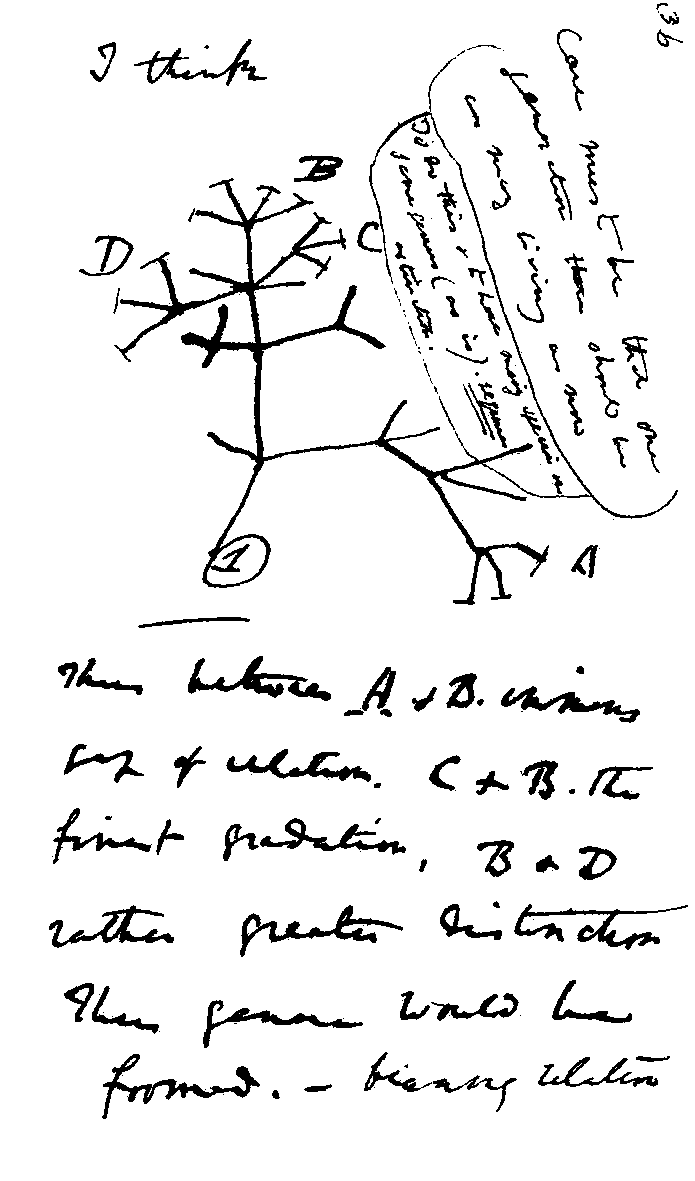
\includegraphics[width=\textwidth]{title} % Note: image is 695 X 1,181 pixels
\end{minipage}
\hfill
\begin{minipage}[b]{0.35\textwidth}
  \begin{flushright}
    \footnotesize
    \textit{``A measure of wisdom | each man shall have,\\
    But never too much\\let him know;\\
    For the wise man's heart | is seldom happy,\\
    If wisdom too great he has won.''} \\
    --- \textit{H\'avam\'al}, 55 
  \end{flushright}
  \vspace{2cm}
\end{minipage}

\clearpage

\onehalfspacing

All living things exist in a constant state of conflict with the biological agents that exploit them in the arena of evolution.
Since the advent of civilization humans have sought an upper-hand in this biological arms race: we harvest the flora and fauna that surround us through agriculture and domestication to our benefit, and we fiercely seek to defeat the plants, animals, and disease-causing pathogens that would do us harm.
While we have largely found means to overcome the challenges of our natural environment to lengthen and improve our lives, the eradication of parasites, bacteria, and viruses remains one of the great challenges facing mankind.
Indeed, as the human population grows and urbanizes we become increasingly vulnerable to new diseases more rapidly than ever before.
Concurrent with the exponential growth and globalization of humans is a demand for increased quality of living; which in turn necessitates the human colonization of natural environments that were previously uninhabited by humans in search of land and resources.
This intrusion into environments puts us into greater contact with animals that host diseases that our species has never before encountered, leading to an ever-increasing risk of emerging infectious diseases (\gls{eid}s) jumping from their natural reservoir into human beings, and spreading at unprecedented speeds through their new susceptible hosts.
Perhaps the greatest of these threats is that posed by viruses.

Viruses are the root cause of some of the \gls{eid}s that have caused the most human suffering and death over the last hundred years.
They have been responsible for outbreaks that have affected local regions (e.g. Ebola virus in central and western Africa \& MERS-CoV in the Arabian peninsula) to epidemics that can seasonally threaten large portions of the globe (e.g. Dengue virus, RSV, and West Nile Virus) to pandemics of global scale that threaten all people (e.g. seasonal influenza viruses, \gls{hiv}, and \gls{sarscov2}).
In fact, viruses have been responsible for all major pandemics since the year 1900: six major influenza pandemics (ranging from the 1918 Spanish flu to the 2009 H1N1pdm09 ``swine flu''), the \gls{hiv}/AIDS pandemic beginning in 1981, and the 2020 COVID-19 pandemic.
Viruses also have some of the greatest future pandemic potential due to their ubiquity and fast-mutating nature.

Fortunately, global public health efforts have made increasingly effective strides toward understanding and eliminating viral pathogens, perhaps most famously by eradicating smallpox through a global vaccination campaign ending in the 1980.
A crucial step in the fight against viral pathogens has been the development of clinical and statistical methodologies that link the outcomes of viral epidemics (case counts, mortality rates, etc.) to the underlying determinants of pathogen spread that drive the epidemic---a field of study known as \textbf{epidemiology}.
While traditional epidemiology has provided invaluable insights, the advent of molecular techniques and the ever decreasing cost of full-genome sequencing has revolutionized our understanding of viral dynamics.
This dissertation illustrates three use cases of how these molecular data can be integrated with traditional epidemiological methods---with a particular focus on \gls{sarscov2} and hepatitis B virus---demonstrating the broad applicability of these techniques in understanding and combating viral epidemics across several different clinically-important time scales.

% 1.1
% NOTE to Guy&Mandev: This section is a bit flowery, but my intention is to get the reader thinking about the interplay of viruses and time
% since that "phylodynamics at time scales" idea is the through-thread of my dissertation
\section{Viral epidemics}\label{sec:int-viralEpi}
Viral epidemics have shaped human history for millennia, leaving their mark on societies and civilizations throughout the ages.
These microscopic pathogens demonstrate an unparalleled ability to spread rapidly through populations, causing widespread illness, death, and social disruption.
From ancient times to the modern era, viruses have been silent yet powerful actors in the drama of human existence, influencing demographics, economies, and even the outcomes of wars.

The historical record is filled with examples of devastation caused by viral epidemics.
In the \nth{5} century BCE, the Plague of Athens decimated the population the eponymous city-state, altering the course of the Peloponnesian War \citep{thucydides1972history}.
Modern-day analysis suggests that this plague may have been caused by a viral hemorrhagic fever \citep{olson1996thucydides}.
The globalization of human movement over the ensuing centuries facilitated the spread of viral pathogens across continents, leading to the emergence of pandemics that reshaped the course of human history.
The arrival of smallpox in the Americas in the \nth{16} century had catastrophic consequences for indigenous populations, facilitating European colonization and reshaping the New World's demographic landscape.
More recently still, the 1918 influenza pandemic, which claimed an estimated 50 million lives worldwide, stands as a stark reminder of the potential for viral pathogens to cause global calamity.

Up to the present, viral epidemics continue to pose significant challenges to global public health and socioeconomic stability.
The \gls{hiv}/AIDS pandemic, first recognized in the early 1980s, has claimed millions of lives and continues to affect communities worldwide.
The emergence of novel coronaviruses, including SARS in 2003 and \gls{sarscov2} in 2019, has demonstrated the ongoing threat of emerging viruses and their potential to rapidly spread in our interconnected world.
As humans continue to expand our built environment into previously uninhabited regions of the planet, we increase the likelihood of zoonotic (animal derived) spillover events, with pathogens such as avian influenza viruses, animal coronaviruses, or poxviruses currently posed as potential threats to future human health if we do not make efforts to hinder their potential jumps into the human population.
These events underscore the critical importance of understanding viral pathogens, their mechanisms of transmission, and their evolution to effectively combat future epidemics and minimize their impact on human society.

\subsection{Epidemics and pandemics}\label{sec:epidemicsVsPandemics}
The ensuing chapters of this dissertation will explore the evolutionary dynamics of viral pathogens across different spatiotemporal scales.
Before delving into the specifics of these analyses, it is helpful to define the terms ``epidemic'' and ``pandemic,'' and to outline the key distinctions between these two related concepts.

An \textbf{epidemic} refers to the occurrence of a disease that exhibits a frequency clearly in excess of normal expectancy within a specific community, geographical area, or season.
Epidemics are characterized by the rapid spread of disease across a particular population or region.
The threshold for declaring an epidemic is context-dependent, taking into account factors such as the pathogen's baseline prevalence, population susceptibility, and local health infrastructure.
Epidemics can vary in scale and duration, ranging from localized outbreaks affecting a single community to more widespread occurrences that impact multiple regions within a country or neighboring nations.

In contrast, a \textbf{pandemic} represents a more extensive and severe form of epidemic, typically characterized by the global spread of a novel pathogen or a new strain of an existing pathogen to which the human population has little to no preexisting immunity.
Pandemics transcend international boundaries, often affecting multiple continents simultaneously and causing sustained community-level outbreaks.
The declaration of a pandemic by health authorities, such as the World Health Organization, considers not only the geographical extent of disease spread but also the severity of the illness and its societal impact.
Pandemics often result in significant morbidity and mortality on a global scale, strain healthcare systems worldwide, and can lead to severe socioeconomic disruptions across affected regions.

In this dissertation, I focus on the evolutionary dynamics of \gls{sarscov2} and hepatitis B virus, two viral pathogens that have had a profound impact on human health and society, however the analyses presented herein consider such dynamics in \textit{specific contexts}.
The coronavirus disease 2019 (COVID-19) pandemic, caused by \gls{sarscov2}, was declared to be a pandemic by the World Health Organization on 11 March 2020 \citep{healthorganization2020coronavirus}, however the analyses described in Chapter~\ref{ch:chapter1} and Chapter~\ref{ch:chapter2} explore the phylodynamics of only the early COVID-19 epidemic in Belgium, and the Omicron epidemic in Pakistan, respectively.
The results of these analyses therefore cannot be extrapolated to the global dynamics of the COVID-19 pandemic as a whole.
Chapter~\ref{ch:chapter3} explores the evolutionary history of hepatitis B virus, which is not considered to be an epidemic or pandemic in the traditional, but is rather endemic to the human population in most of the world.

\subsection{Traditional and genomic epidemiology}\label{sec:tradVsGenEpi}
The field of epidemiology has long been concerned with understanding the spread of infectious diseases and the factors that influence their transmission.
Traditional epidemiological methods, such as contact tracing, case reporting, and mathematical modeling, have been instrumental in controlling outbreaks and informing public health interventions for hundreds---if not thousands---of years.
One of the earliest examples of epidemiological investigation dates back to a 1854 cholera outbreak in the West End of London, where Dr. John Snow correlated counts of cholera cases at different addresses to nearby water sources.
By making such a correlation, he was able to identify a contaminated water pump on Broad Street as the putative source of the epidemic (Fig.~\ref{fig:broadStreetPump}).

\begin{figure}[ht]
  \centering
  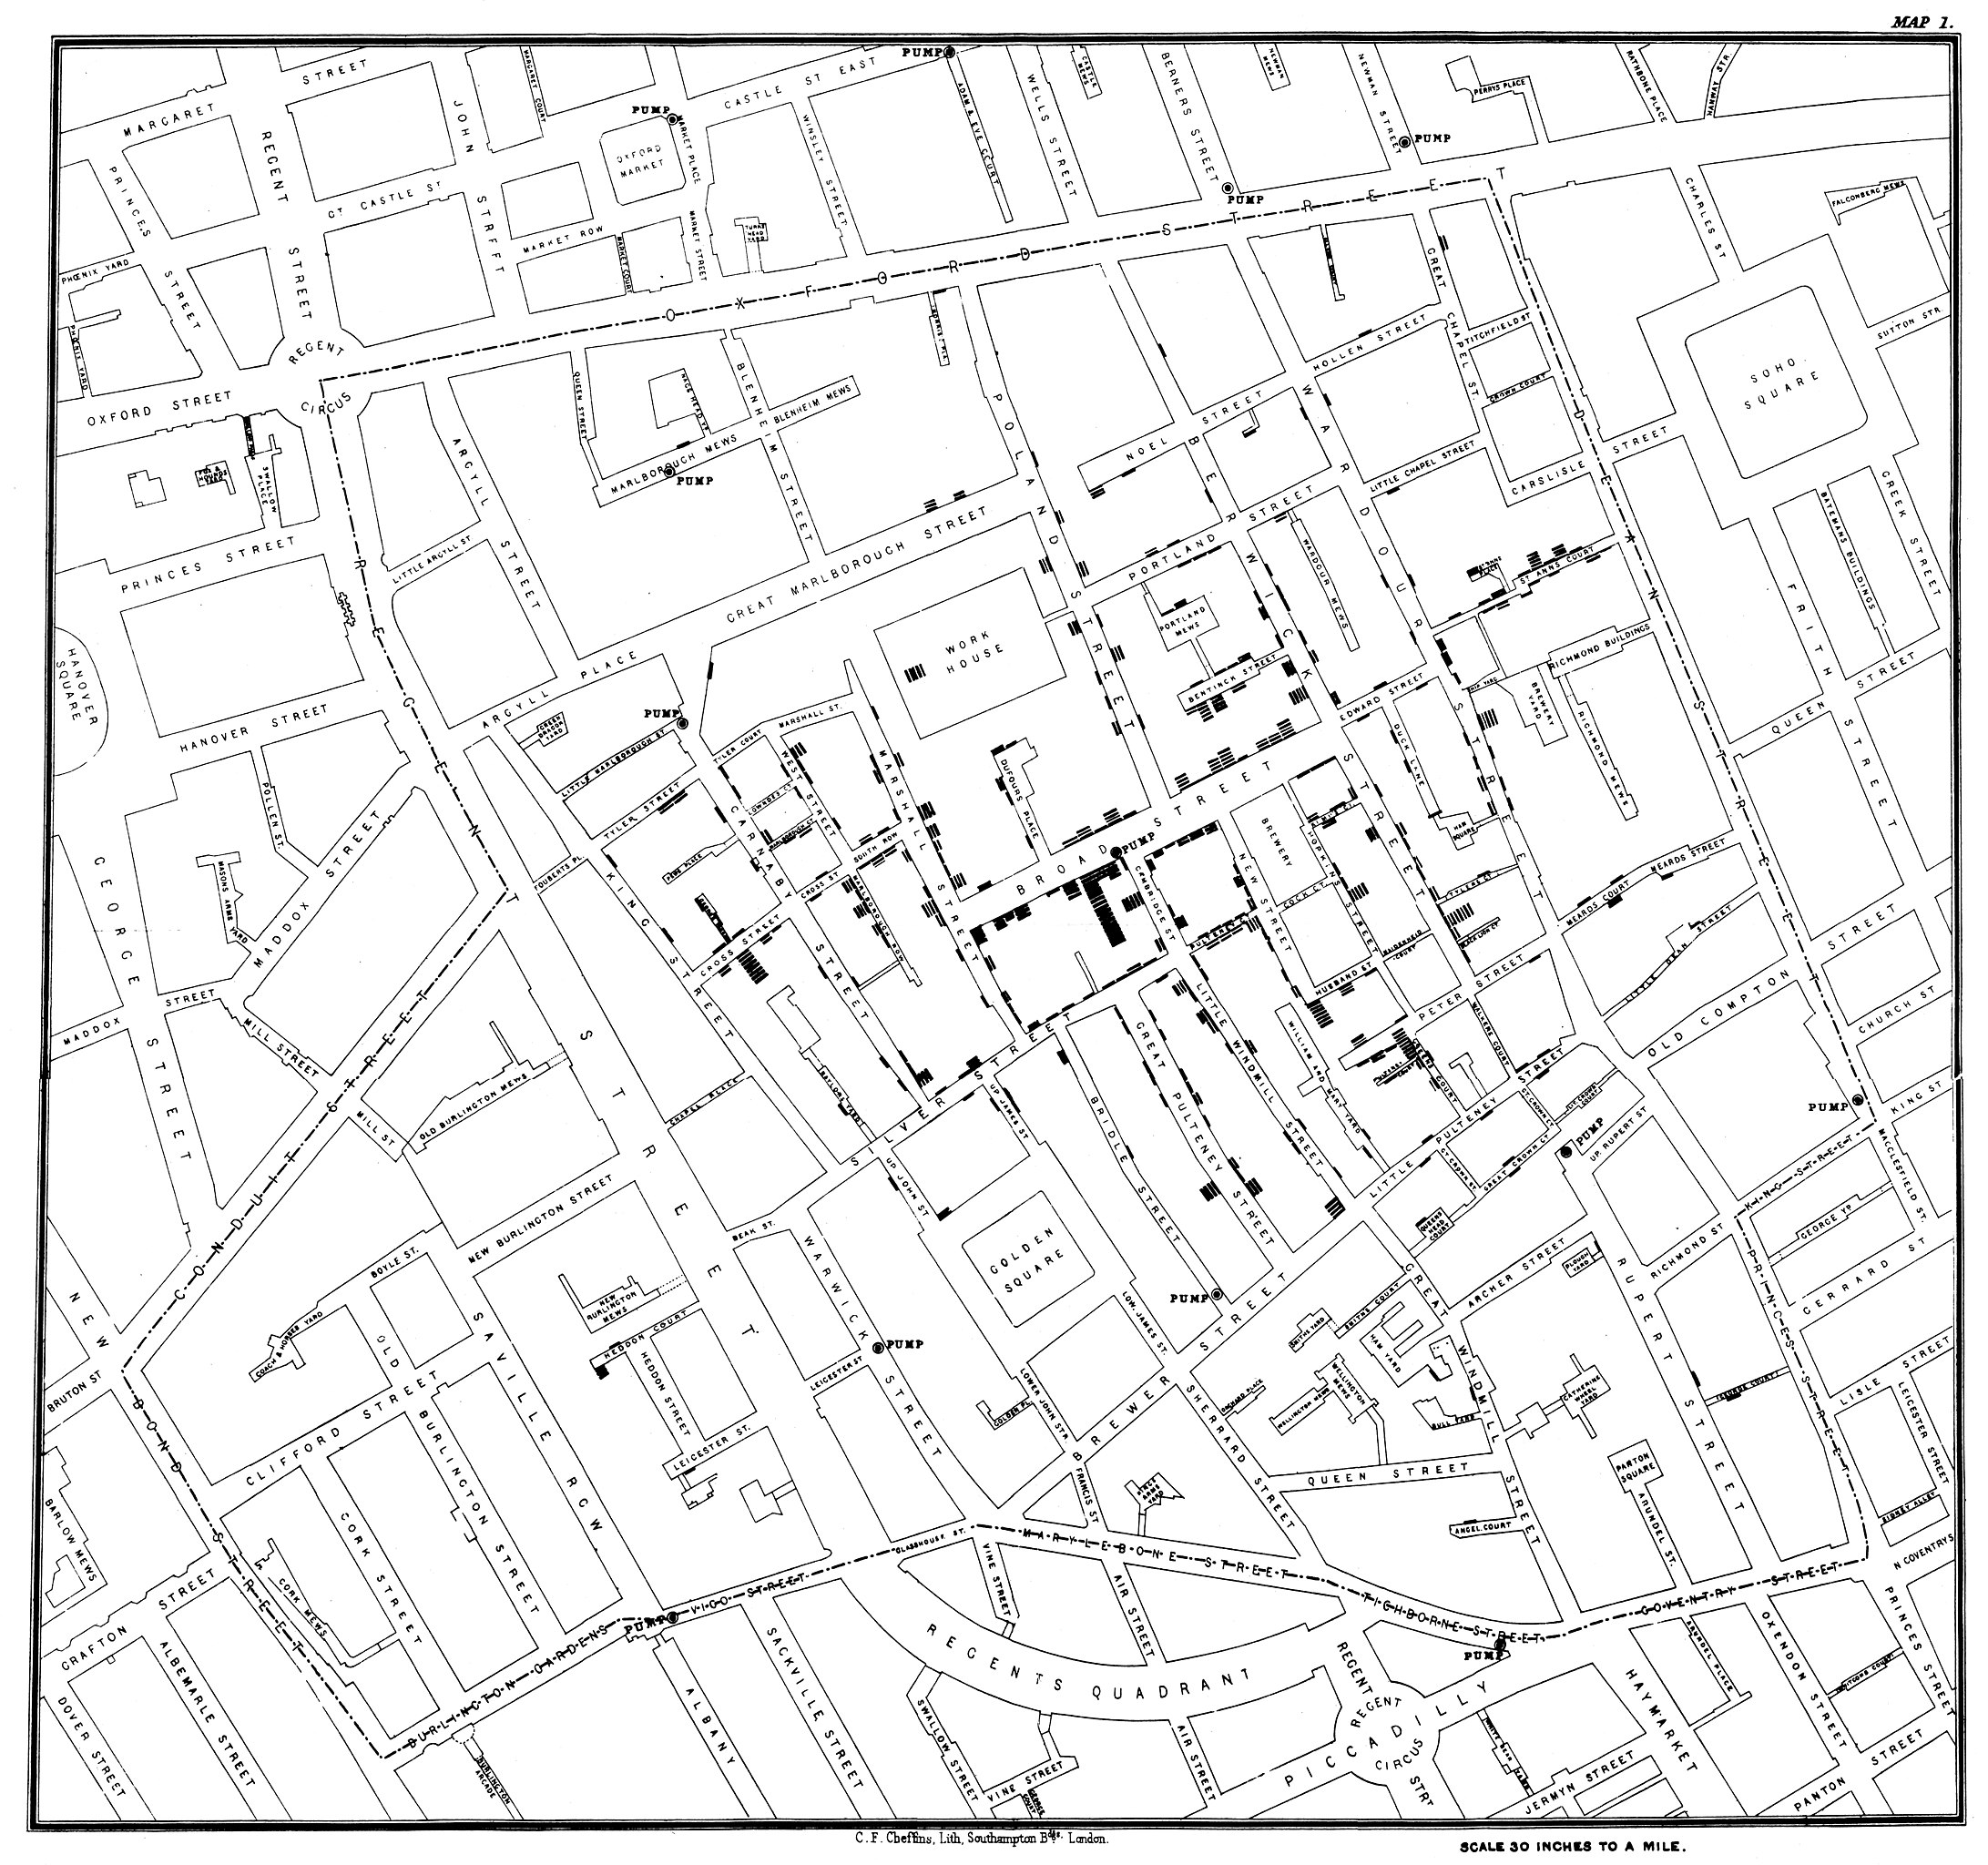
\includegraphics[width=.6\textwidth]{broad_street_pump}
  \caption[John Snow's map of the 1854 Broad Street cholera outbreak in London]{John Snow's characterization of the 1854 London cholera outbreak is considered epidemiology's foundational moment. Snow incorporated the geographic locations (addresses) of Snow's map of the outbreak, which showed a cluster of cases around the Broad Street pump, illustrates the process that led him to conclude that the pump was the source of the outbreak. \textit{Figure credit: John Snow, 1854} \citep{snow1854mode}.}
  \label{fig:broadStreetPump}
\end{figure}

In the years since Snow's pioneering work, epidemiology has evolved into a multidisciplinary field that combines elements of medicine, public health, statistics, and social science to study and determinants of health and disease in populations.
Epidemiological methods have been instrumental in controlling infectious diseases, identifying risk factors for disease transmission, and evaluating the effectiveness of public health interventions.
Indeed, as technology and data collection methods have advanced, epidemiologists have been able to develop increasingly sophisticated models of how diseases spread.

At the core of most epidemiological models lie three main data components: identified infections, locations, and times.
These three basic components can be combined in a number of ways to build more complex descriptions of disease spread (e.g. epidemic curves, spatial maps of disease incidence, etc.).
Both on their own and combined with other sources (patient demography, clinical interventions and outcomes, etc.), these data can be input into extremely robust models that can be used to not only retrospectively describe epidemics, but also to make predictions about future spread that can be used to inform public health policy.

However, following the discovery of the structure of DNA by Rosalind Franklin, James Watson, and Francis Crick in 1953 \citep{franklin1953molecular,watson1953molecular}, the field of epidemiology has been revolutionized by the advent of molecular techniques.
The addition of molecular data gave epidemiologists a newfound ability to not just analyze the disease outcomes that are can be observed in a population, but also to analyze the biological agents directly responsible for the epidemics.
The field was further revolutionized in 1976, with the first full-genome sequence of a virus \citep{fiers1976complete}.
As sequencing technology has become more advanced and less expensive, we now have the ability to obtain full-genome sequences of viral pathogens from hundreds or thousands of infected individuals in a single outbreak, allowing us to compare genetic sequences (Fig.~\ref{fig:alignment}) through an assortment of methodologies.
When these methods are applied to pathogen outbreaks in an effort to understand the dynamics of the pathogen and inform public heath interventions, we refer to them collectively by the name of \textbf{genomic epidemiology} \citep{armstrong2019pathogen,black2024applied}.

Though there are parallels between them---and they often address similar underlying biological questions---traditional epidemiology and genomic epidemiology represent complementary approaches to understanding disease spread and dynamics, each offering distinct insights into public health challenges.
While both methodologies seek to understand patterns of disease occurrence and transmission, they differ fundamentally both their primary units of analysis, and in their ultimate research goals.
Traditional epidemiology focuses on infected individuals and population-level health outcomes, examining factors such as disease incidence, prevalence, mortality rates, and risk factors---these methods can be applied to both infectious and non-infectious diseases.
It has a long history of helping researchers and public health officials understand disease burden, identify vulnerable populations, and implement public-health interventions.
By contrast, genomic epidemiology focuses on the heritable characteristics of disease-causing pathogens themselves.
By examining the genetic signatures of pathogens as they spread through populations, genomic epidemiology can help us to better understand transmission chains, identify the emergence of novel variants, and to track the evolution of virulence or drug resistance---questions that may be difficult or impossible to address through traditional epidemiological approaches alone.

\begin{figure}[ht]
  \centering
  \begin{subfigure}{0.95\textwidth}
    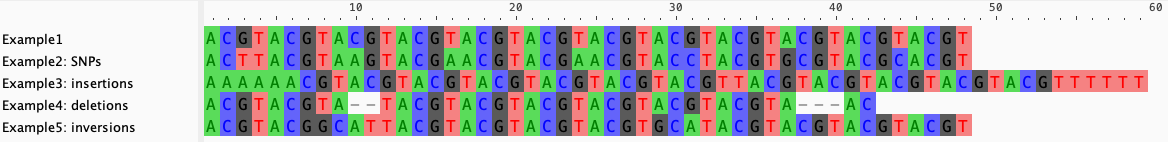
\includegraphics[width=\textwidth]{unaligned}
    \caption{}
  \end{subfigure}
  \begin{subfigure}{0.95\textwidth}
    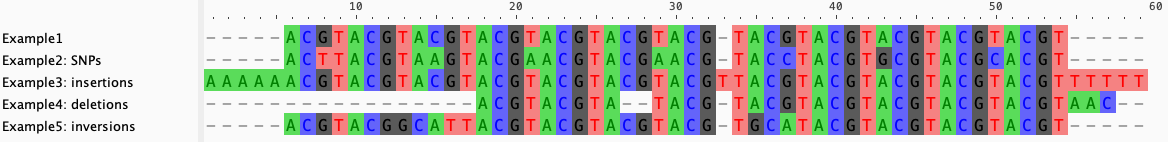
\includegraphics[width=\textwidth]{aligned}
    \caption{}
  \end{subfigure}
  \caption[Multiple sequence alignment]{A set of five example genomic sequences viewed both \textit{(a)} prior to alignment, and \textit{(b)} after being aligned using MAFFT \citep{katoh2013mafft} and visualized using AliView \citep{larsson2014aliview}; each row represents a single sequence, and each column represents a site shared between sequences. Sites are colored by the amino acid present in each sequence at each site. The sequence \textit{Example2} represents the most common type of mutation that we observe: single nucleotide polymorphisms (\gls{snp}s), where a single sequence has a single mutation from one amino acid to another. Examples 3--5 represent other types of genomic motifs that are frequently observed, but not always explicitly modeled by phylogenetic inference algorithms.}
  \label{fig:alignment}
\end{figure}

While there are many different ways that researchers can leverage the information carried in pathogens' genomes to better understand their epidemiological dynamics, this thesis will focus in particular on those dynamics that relate to \textit{shared evolutionary history} of a set of genomic sequences---each representing an individual infected by a virus at a given point in time.
Broadly, our goal is to model evolutionary processes that causes observable differences in pathogen genomes (e.g. Fig.~\ref{fig:alignment}) to hypothesize the patterns of evolution that led to the sequence data that we observe.
We refer to these inferred hypotheses of shared evolutionary history as \textbf{phylogenies}, and the field of research related to their inference as \textbf{phylogenetics}.

\begin{figure}[ht]
  \centering
  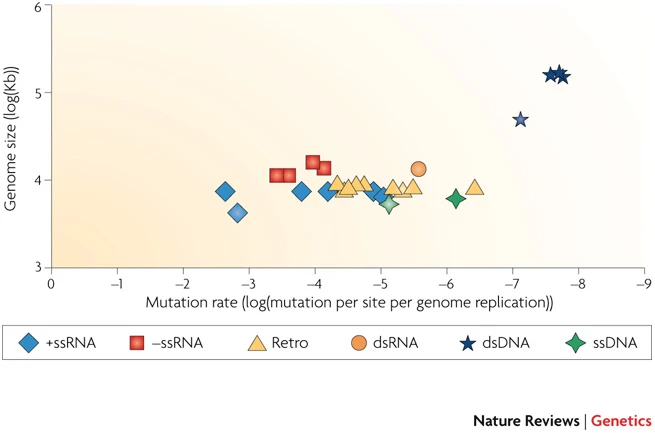
\includegraphics[width=.85\textwidth]{genSizeVsMutRate}
  \caption[Genome size vs. mutation rate in viruses.]{It is a well known phenomenon that as genome size and complexity increases, observed mutation (and evolutionary) rates decrease. For viruses in particular, this has the practical upshot that it means that genomic mutations accumulate frequently enough that they can be found during epidemic timescales. This \bip{finish this sentence} \textit{Figure credit: Duffy, Shackleton, \& Holmes (2008)} \citep{duffy2008rates}.}
  \label{fig:sizeVsRates}
\end{figure}

While it is interesting---and frequently useful---to understand the evolutionary relationships between viral sequences, the inferences made through phylogenetic analysis can tell us much more when we contextualize them in \textit{time} and \textit{space}.
Viruses (and in particular \gls{rna} viruses) accumulate genomic mutations at a staggering rate compared to many other domains of biological entities (Fig.~\ref{fig:sizeVsRates}).
Because of this, we are frequently able to make observations (i.e. collect sequences) of viruses over the same time scales that epidemics play out, and make phylogenetic inferences on the same time scales.
We refer to this merger of phylogenetic and epidemic time scales as \textbf{phylodynamics}.
When viral genomes also come with associate geographic metadata, we are able to make further inferences (either in sequence or jointly with the phylogeny) of where common ancestors of taxa likely existed, and the associated rates of migration between the sampled locations.
This process of combined spatiotemporal and evolutionary inference will be referred from here on as \textbf{phylogeography}.
These concepts are illustrated in Figure~\ref{fig:phylogeneticsOverview}.

\begin{figure}[ht]
  \centering
  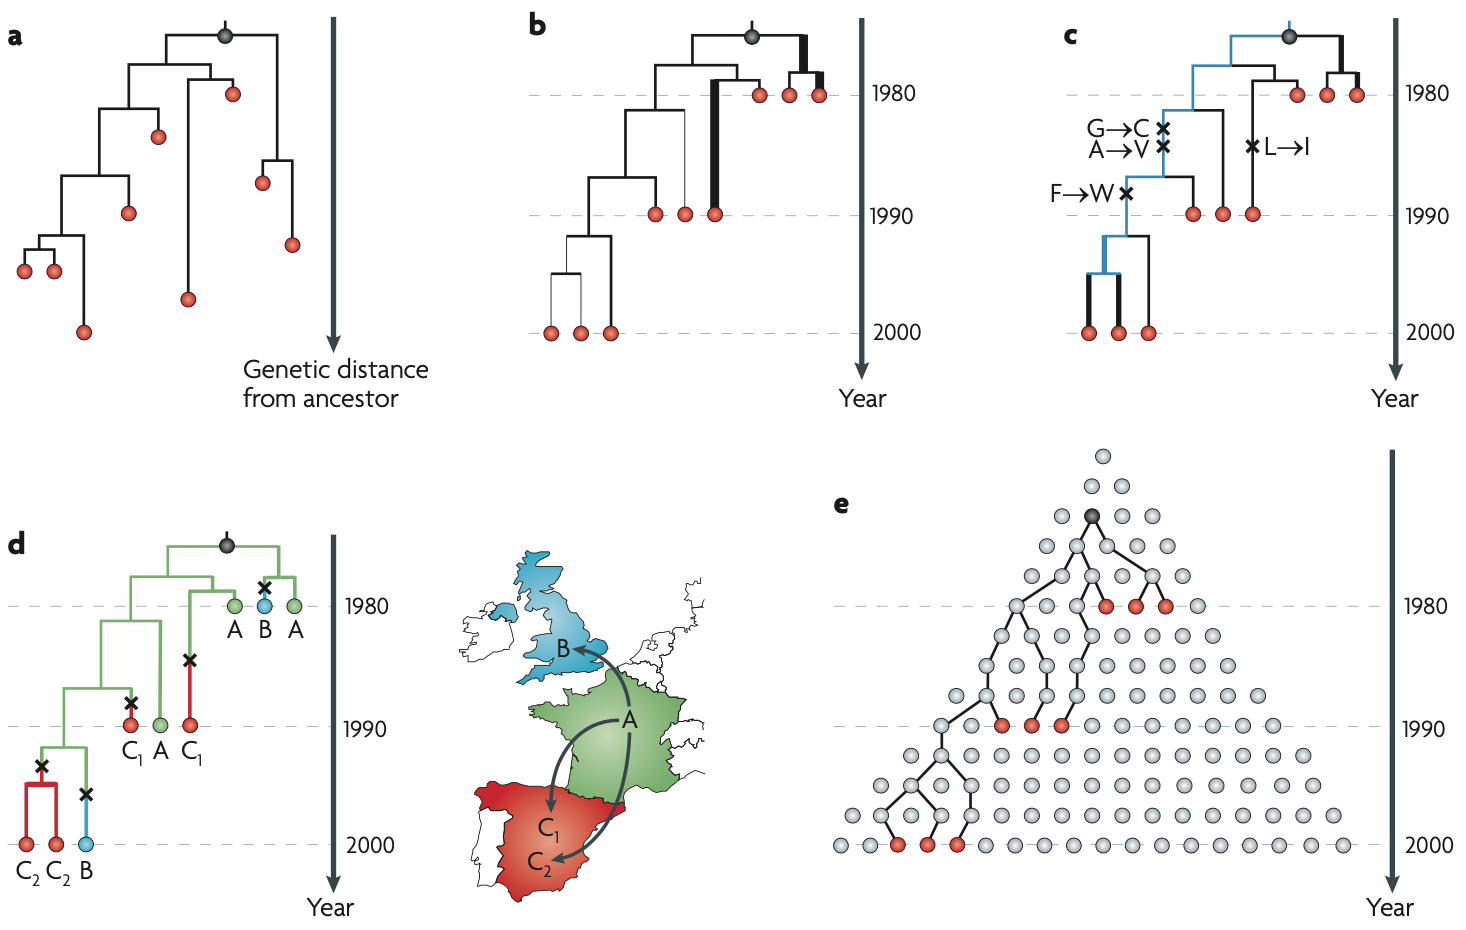
\includegraphics[width=.85\textwidth]{rambautFig}
  \caption[Applications of phylodynamics]{Fundamental concepts in phylodynamic analysis. a) Rooted, bifurcating phylogenetic tree derived from (viral) genomic sequences, branch lengths (here shown on the vertical axis) represent observed genetic distance. b) Time-calibrated phylogenetic tree demonstrating the phylodynamic relationship between genetic distance and time. Branch lengths now represent time. c) Mutations take place along the tree's branches, with mutations that become fixed falling on the backbone tree's (blue) versus those on terminal branches (black) which are not yet fixed in a subpopulation. d) Discrete phylogeographic inference hypothesizes the history of pathogen spread. Branches are annotated by inferred geographic locations. e) Underlying pathogen population structure influences tree shapes. When we consider a tree drawn from a population that varies in size through time, we observe different patters of branching patterns and branch lengths.
  \textit{Figure credit: Pybus \& Rambaut (2009)} \citep{pybus2009evolutionary}.
  }
  \label{fig:phylogeneticsOverview}
\end{figure}

\subsection{A general model of the epidemic process}
In the pursuit of descriptive models for pathogen evolution and spread, it is important to ask, ``Is this model a faithful description of my biological question?''
To answer this question, it is necessary to construct a high-level framework of this biological system (i.e. epidemic spread), and to recognize the assumptions inherent to that framework.
To this end, a brief description of the epidemic process as seen through the lens of phylogenetics is required so that we can answer the question, ``Do molecular phylogenies accurately describe viral epidemics?''

At the beginning of an epidemic, we imagine that there is a single individual who is infected by a virus, and they remain infectious for some limited period of time (either they will recover to the point of no longer being infectious, or die).
During their infectious period, the individual may go on to infect one or more other individuals with the virus (Fig.~\ref{fig:epiProcess}a).
This process is then able to repeat itself for each of the infected individuals, and in turn for individuals infected downstream.
Generally, if on average each infected person spreads the virus to more than one new person the epidemic will grow, and if they spread to fewer than one person on average then the epidemic will shrink.
At some point---or in practice at many points---during the downstream epidemic, individuals may be sampled and a complete viral genomic sequence may be isolated from the individual (Fig.~\ref{fig:epiProcess}b).

Each genome will be similar though slightly different from one other, and the degree to which they differ will be in proportional to how deep in the transmission history the two sequences differ.
Put differently, we expect sequences to be similar in proportion to the amount of evolutionary history that they share (Fig.~\ref{fig:epiProcess}c).
In this model, we assume that transmission events represent a complete (or complete-enough) and instantaneous bottleneck on the population, and that each individual can be represented by a single consensus genomic sequence.
We also assume that evolution takes place independently along each branch of the tree---that is, mutations that occur along one branch of the phylogeny have no affect on the other branches.

\begin{figure}[ht]
  \centering
  \begin{subfigure}{0.45\textwidth}
    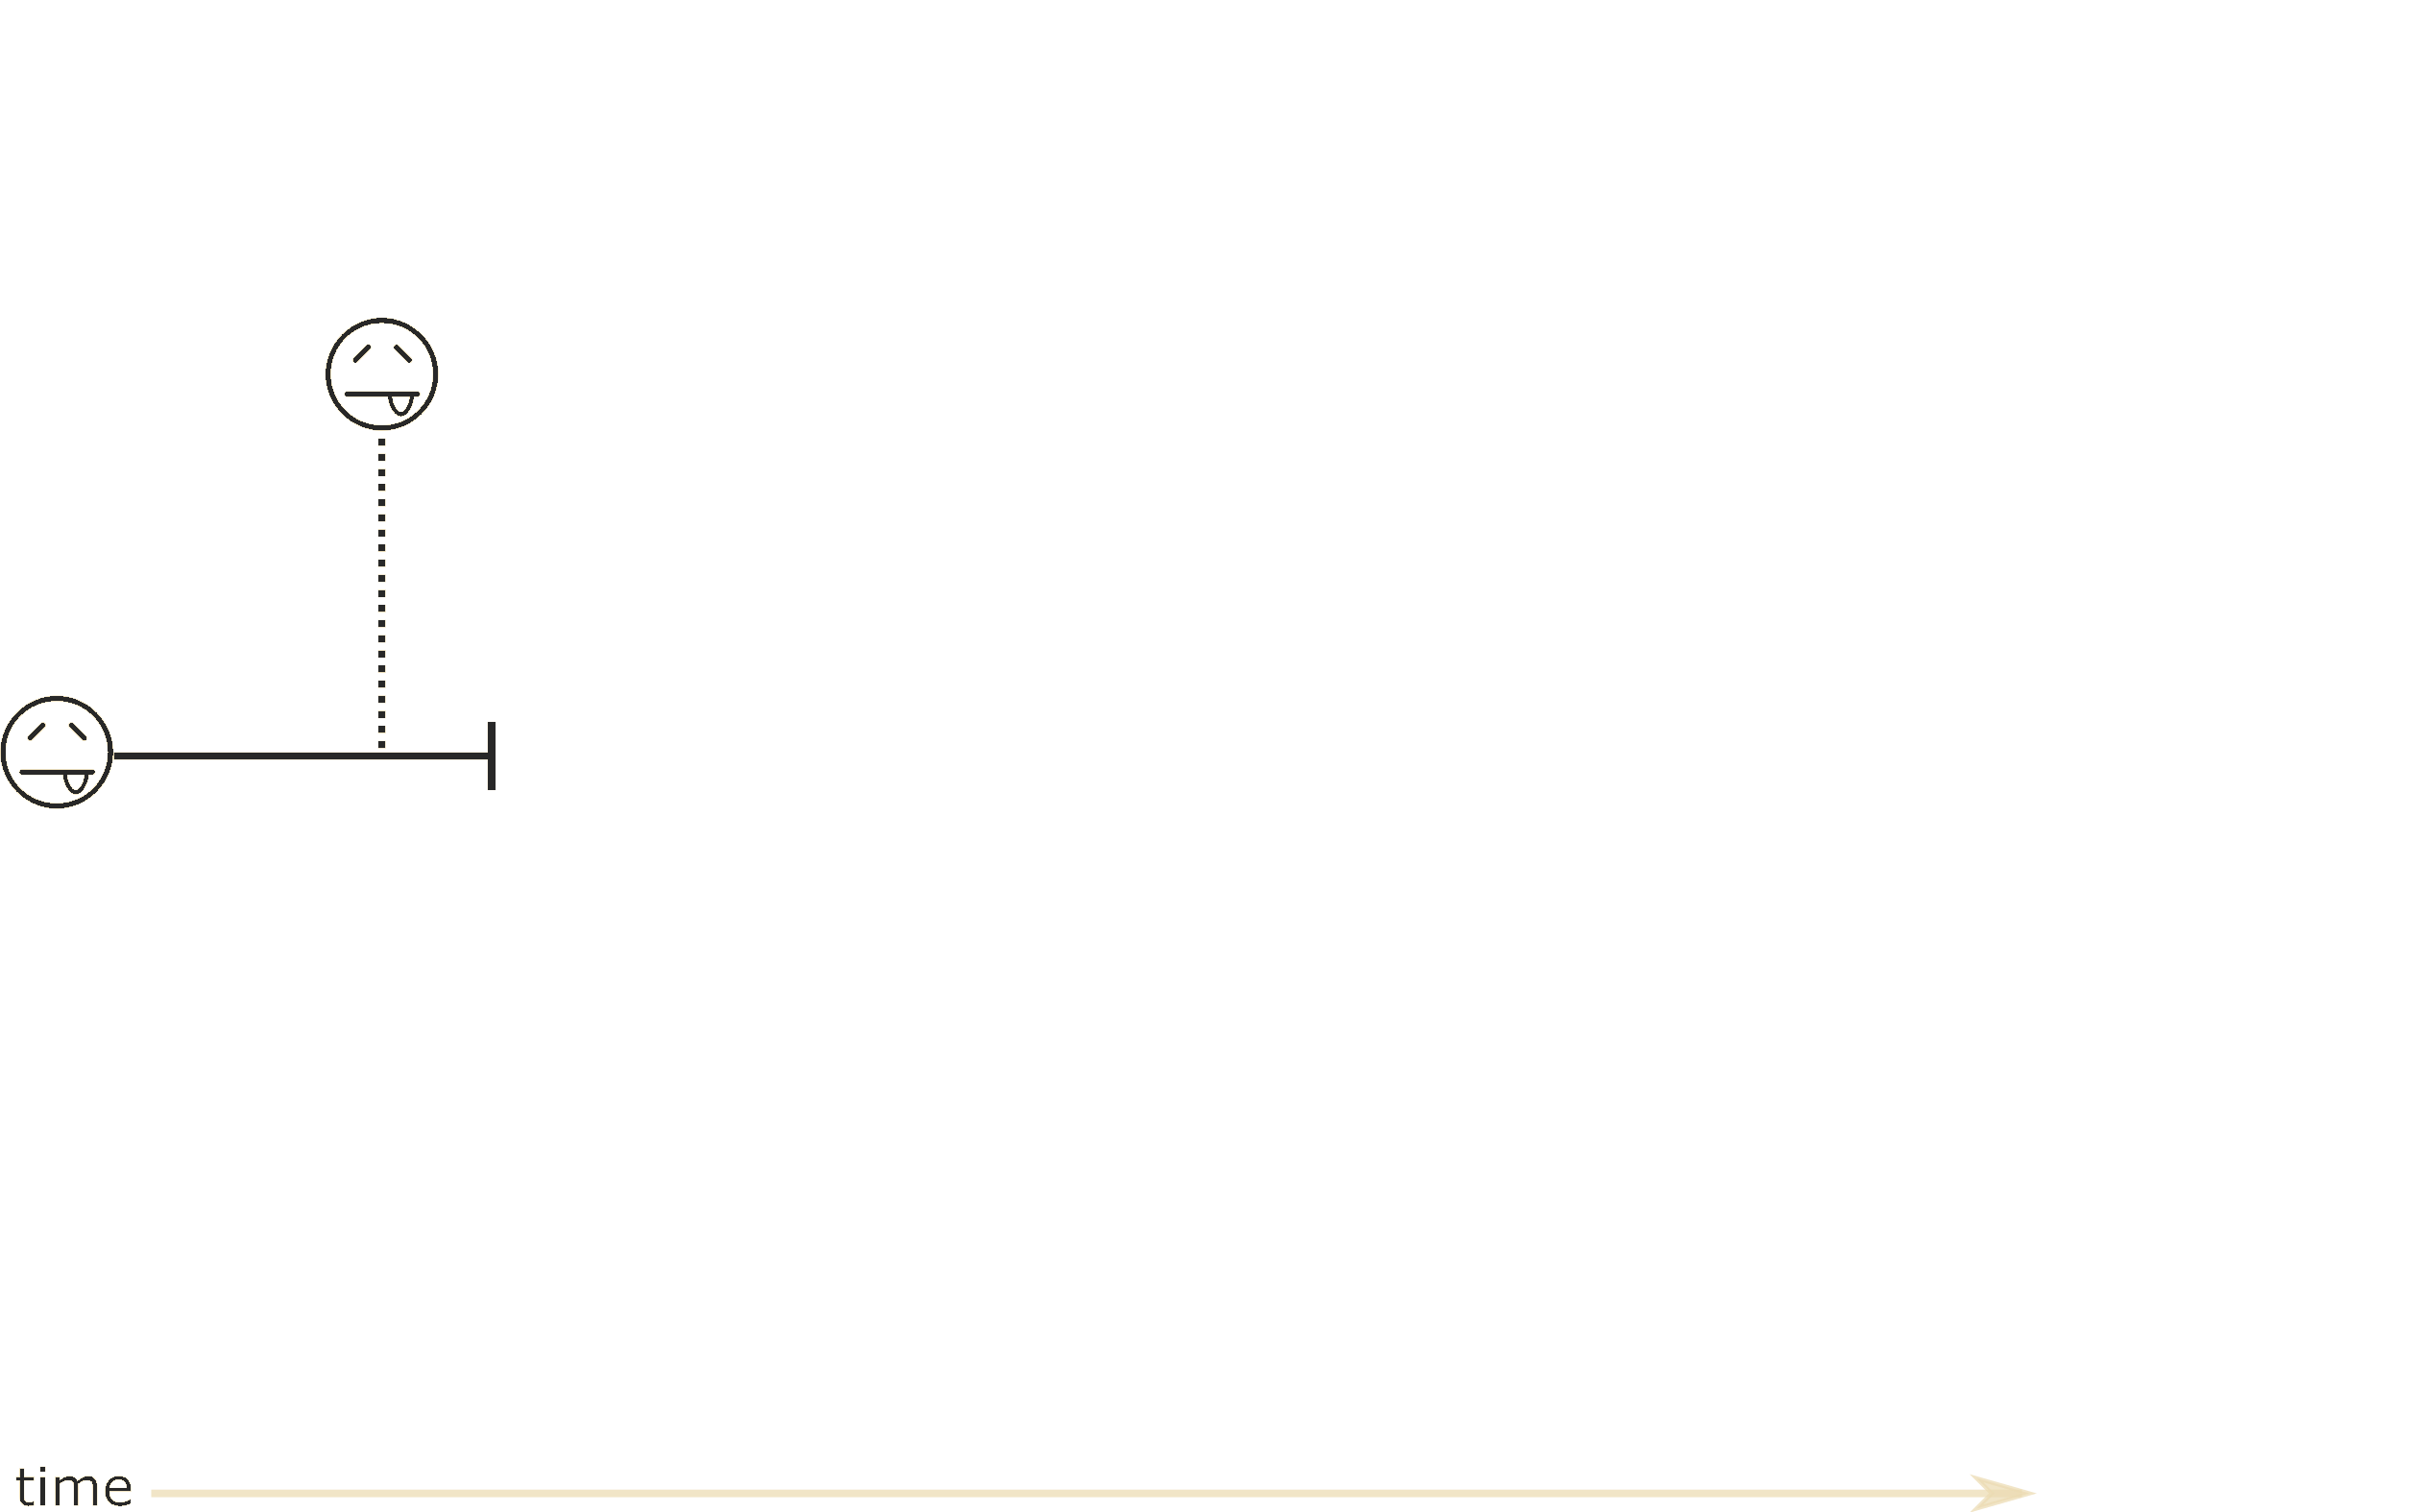
\includegraphics[width=\textwidth]{epi2}
    \label{fig:epiProcess1}
    \caption{}
  \end{subfigure}
  \begin{subfigure}{0.45\textwidth}
    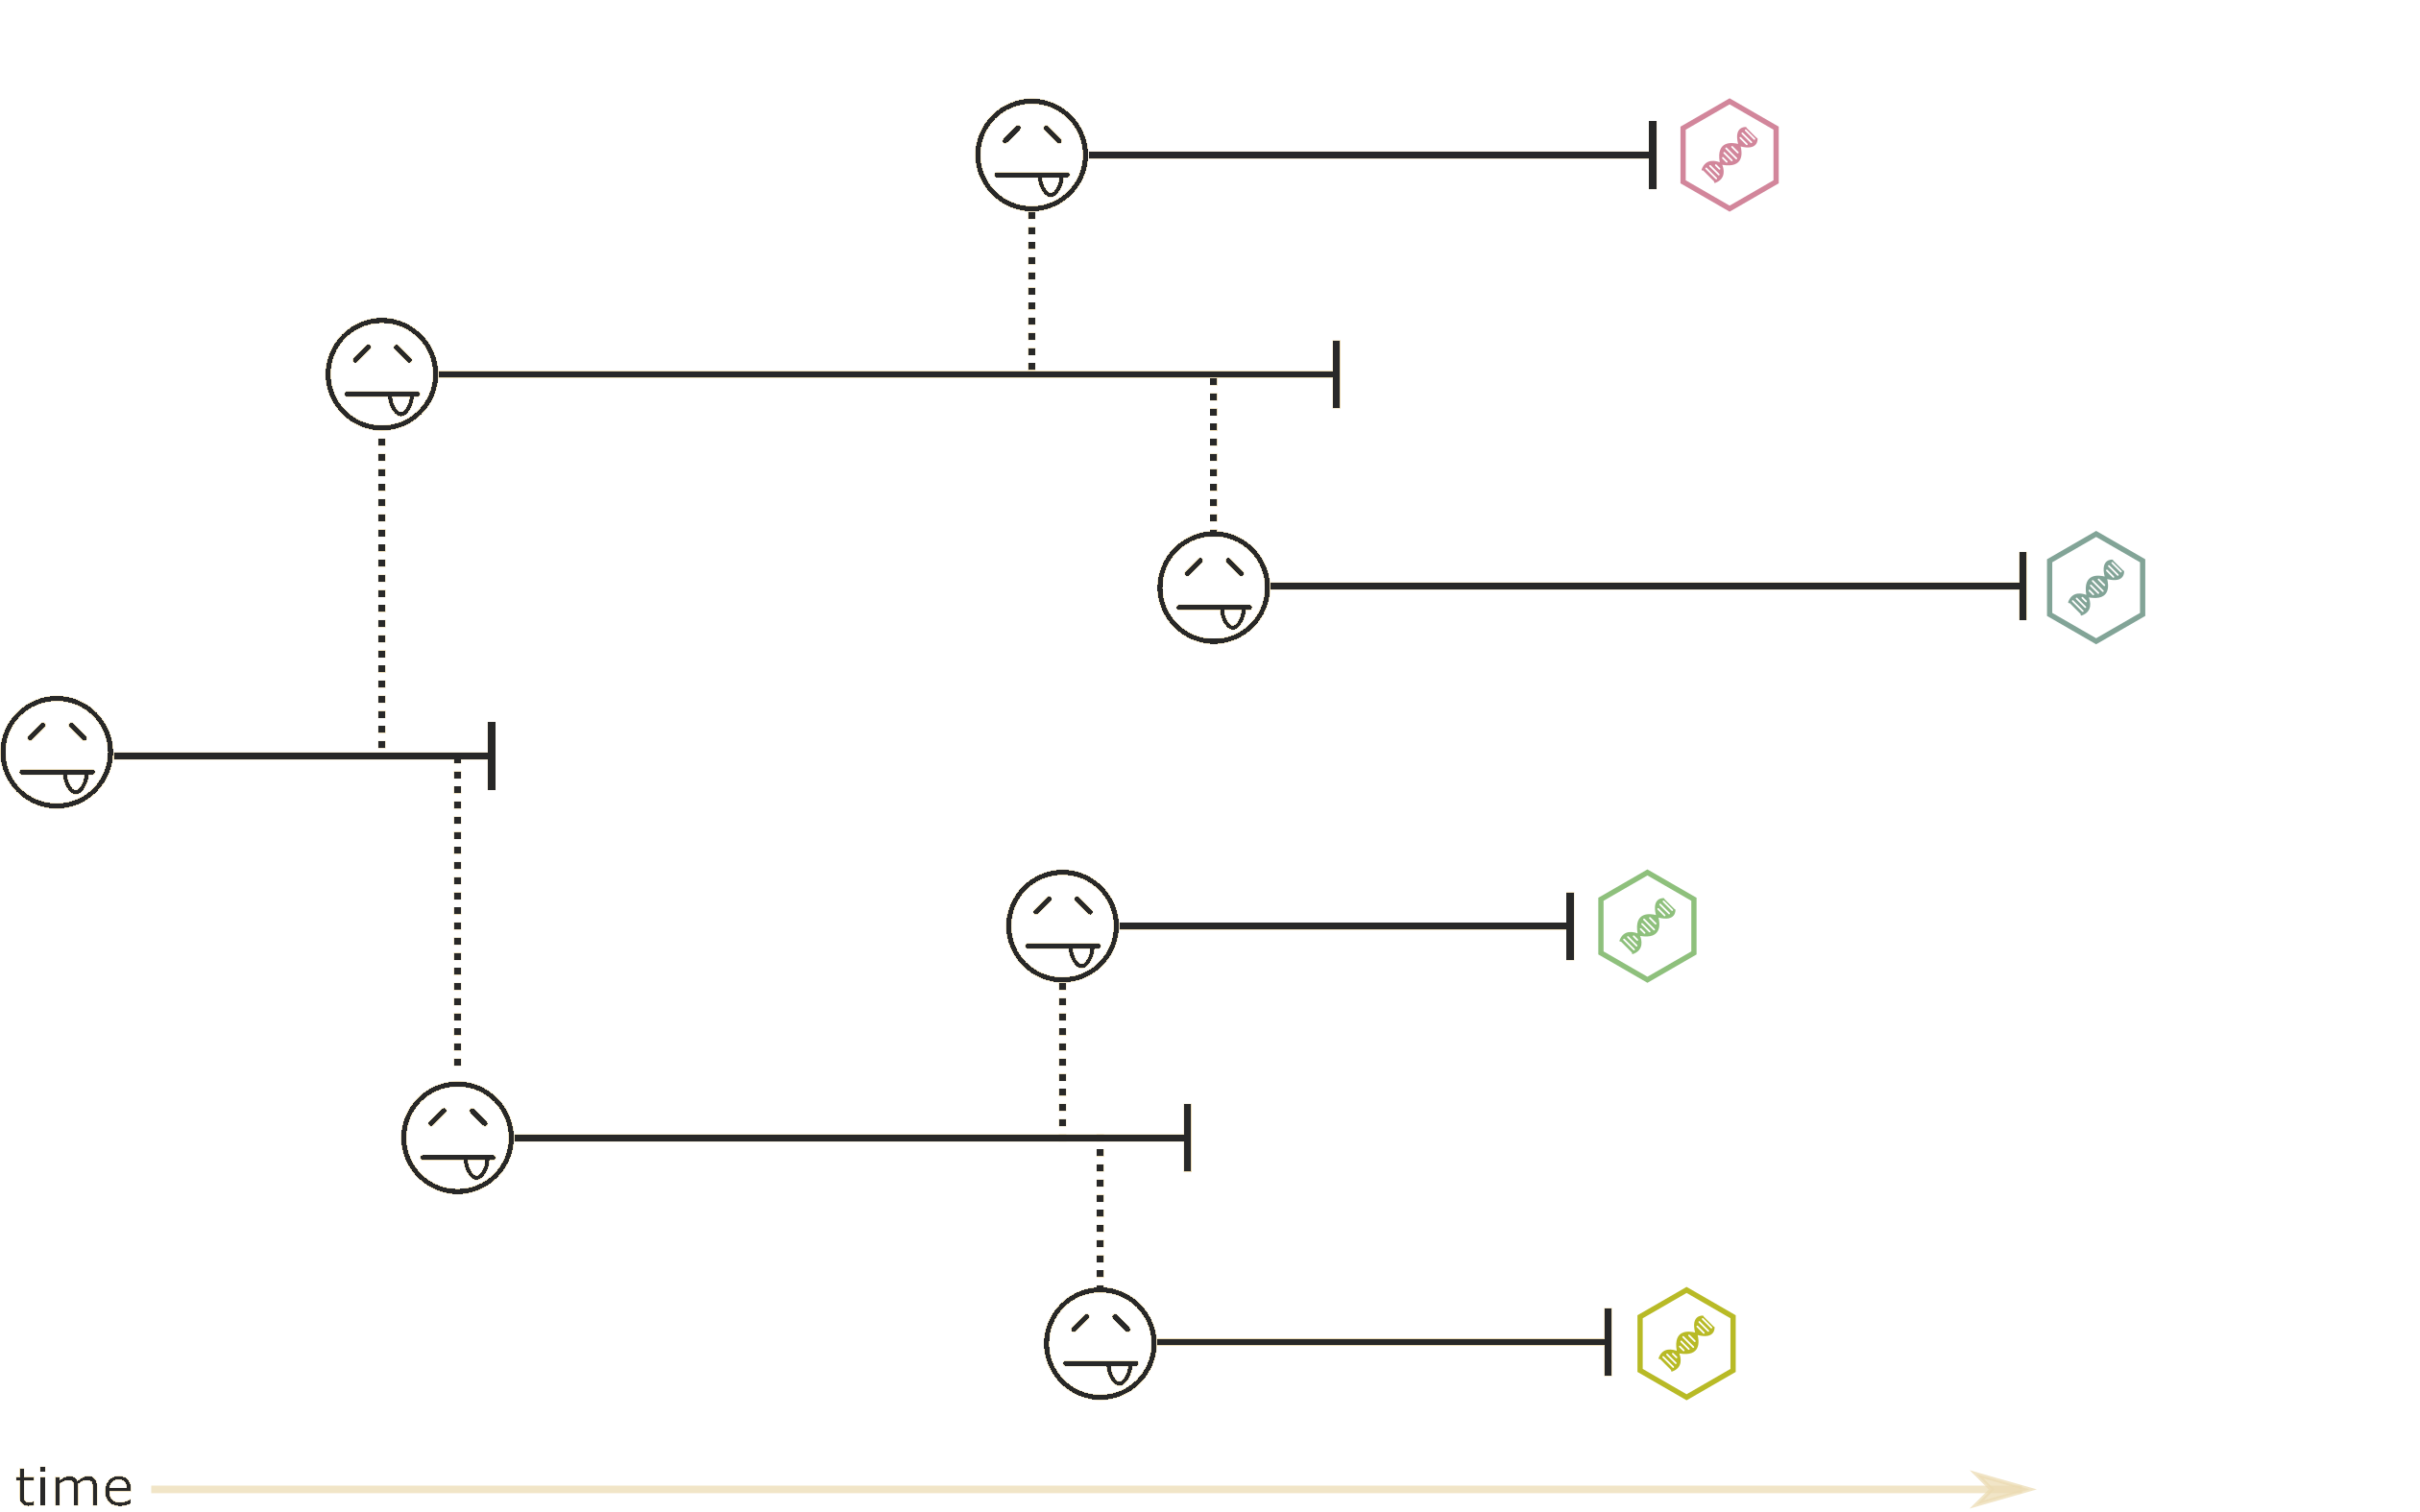
\includegraphics[width=\textwidth]{epi5}
    \label{fig:epiProcess2}
    \caption{}
  \end{subfigure}
  \begin{subfigure}{0.45\textwidth}
    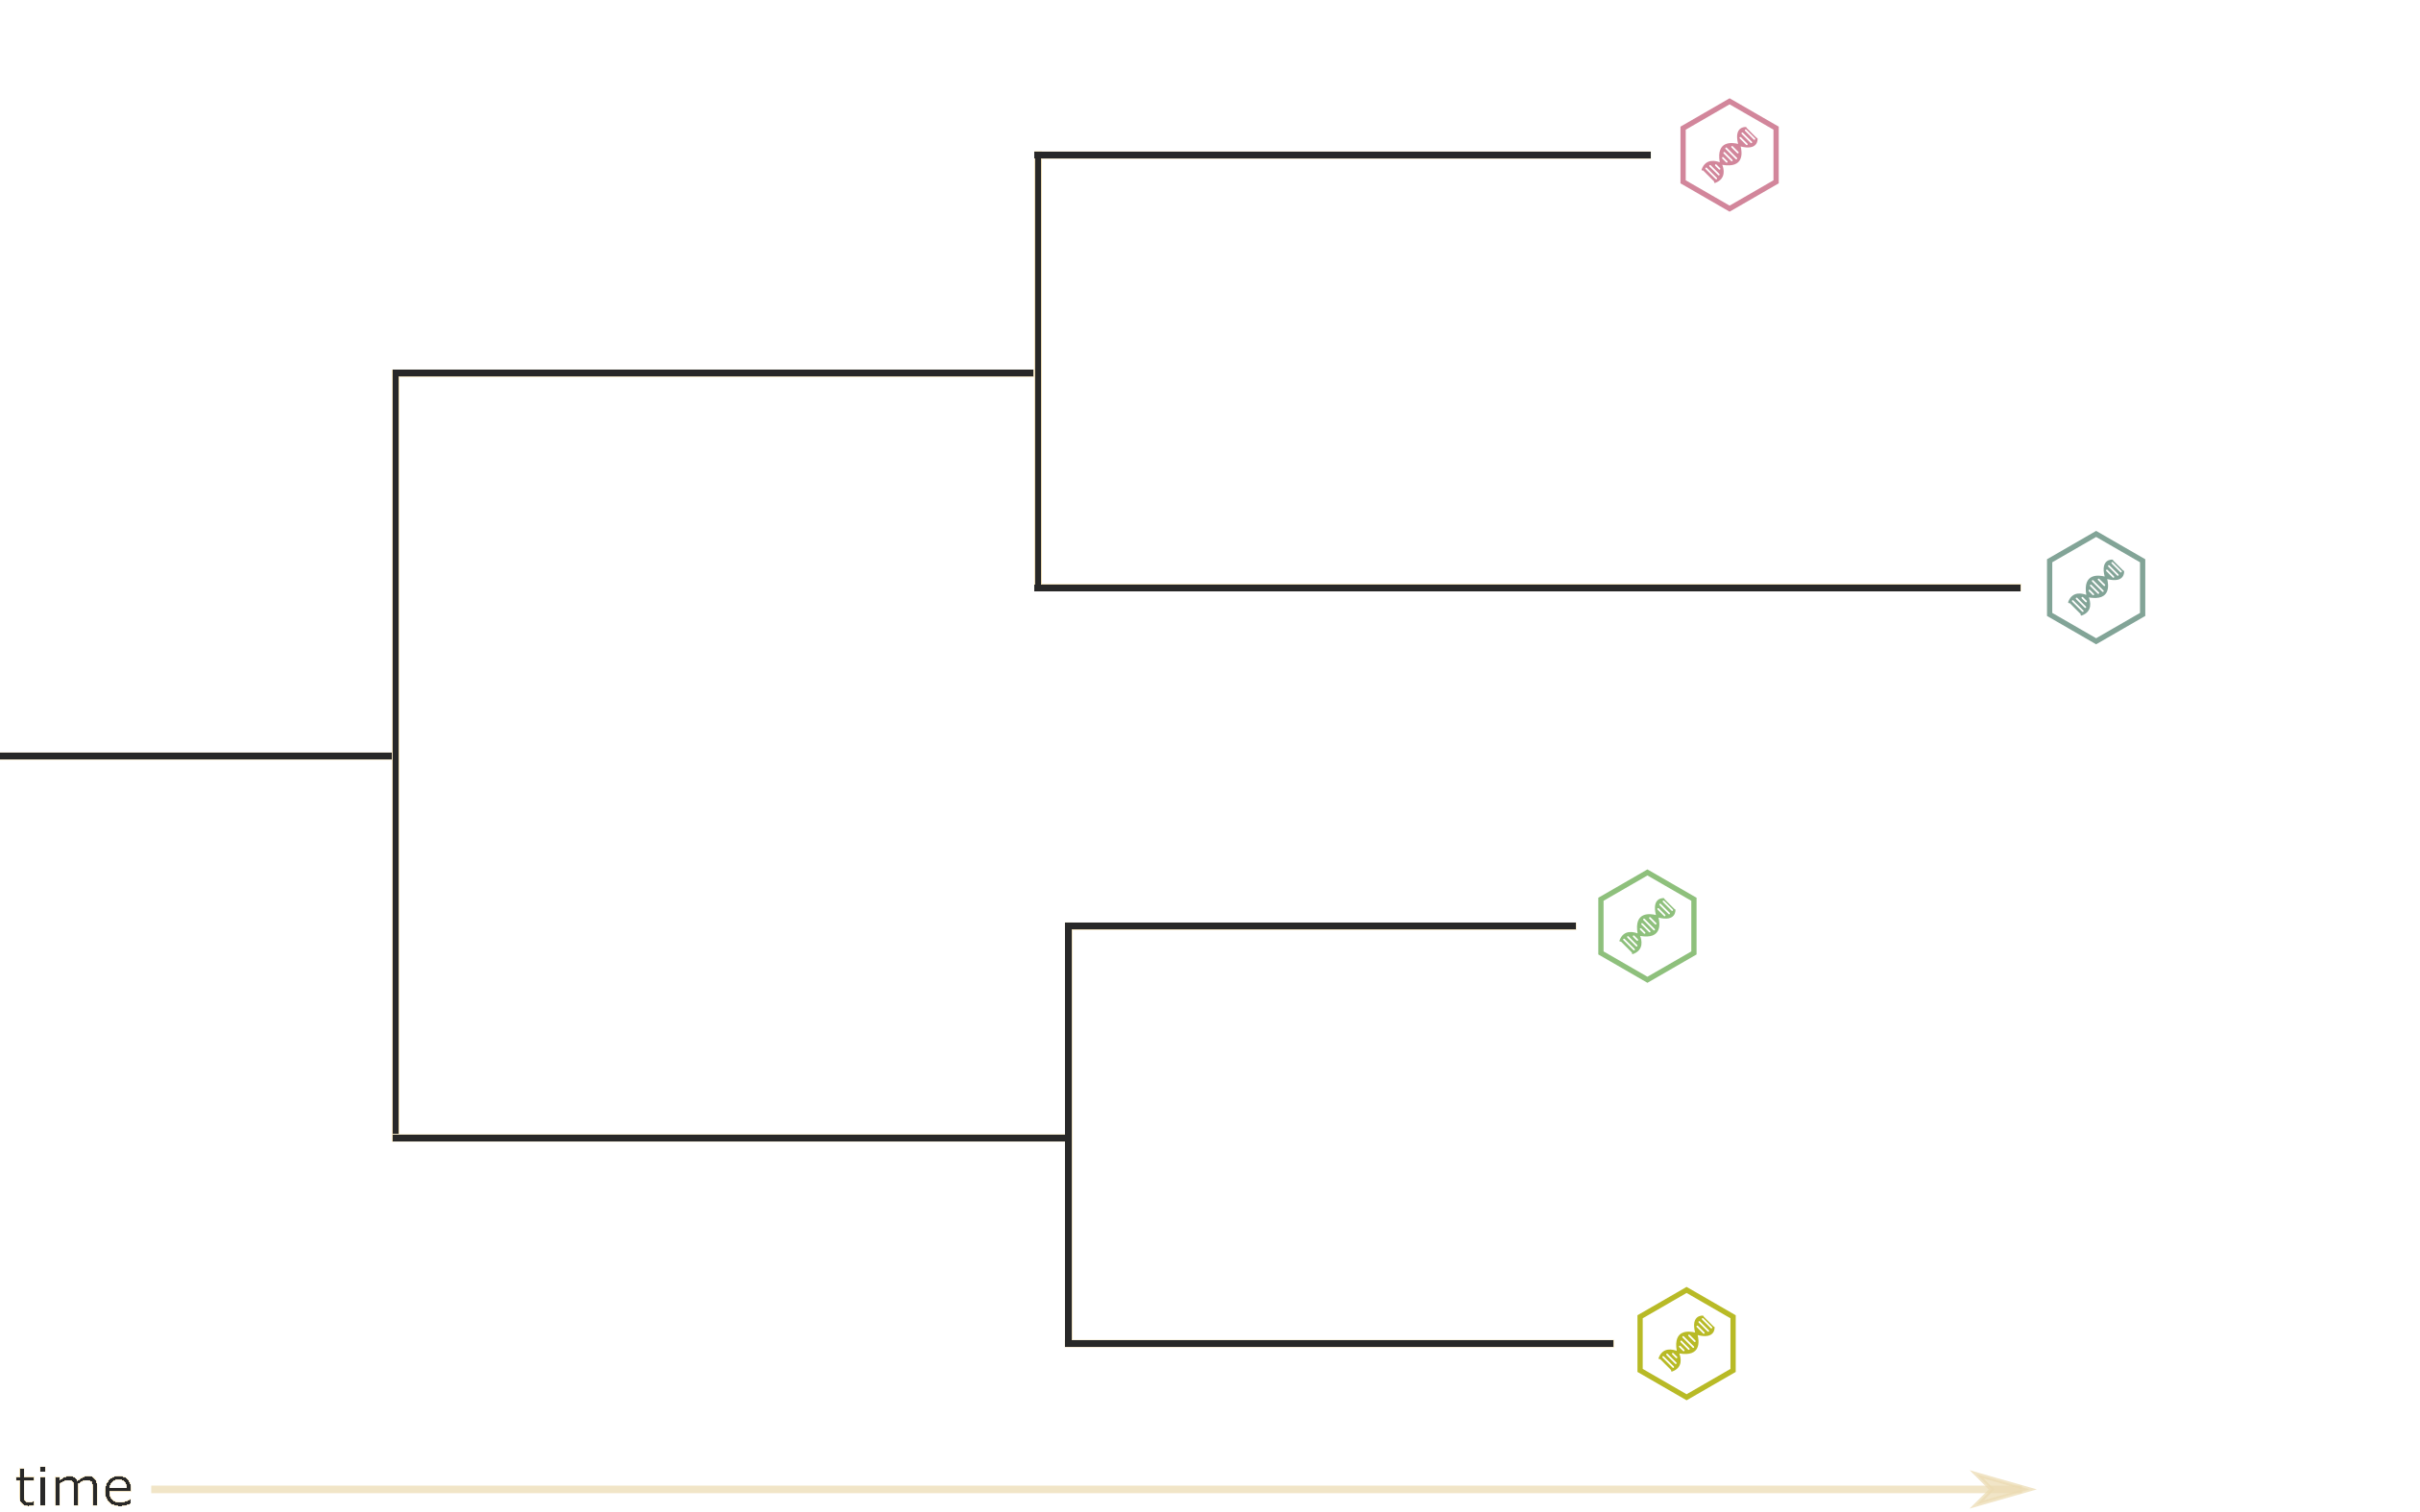
\includegraphics[width=\textwidth]{epi6}
    \label{fig:epiProcess3}
    \caption{}
  \end{subfigure}
  \caption[The epidemic process is inherently treelike]{\textit{(a)} an individual with an infectious period indicated by a solid horizontal line; dashed vertical line indicates an instantaneous infection event. \textit{(b)} Downstream in the epidemic, subsequently infected people are sampled, and genomic sequences are generated from their infecting virus. Viruses that are more closely related (e.g. the two green sequences at the bottom of the tree) have sequences that are more similar to each other than to more distanty related sequences. \textit{(c)} Statistical modeling of the similarities in viral sequences allows us to reconstruct a hypothesis of the shared evolutionary history that links the sequences.}
  \label{fig:epiProcess}
\end{figure}

\subsection{Genomic epidemiology across spatiotemporal scales}
This thesis will explore three different applications of genomic epidemiology to three different cases, each representing a distinctly different temporal scope.
Each of these cases addresses one of the main uses of phylodynamic methodologies: Chapter~\ref{ch:chapter1} concerns real-time public health-facing phylodynamics, Chapter~\ref{ch:chapter2} uses phylogeography in a \textit{post hoc} manner to understand the ongoing dynamics of a viral epidemic, and Chapter~\ref{ch:chapter3} extends this framework to investigate the long-term dynamics of a virus that has been in the human population for thousands of years.

\subsubsection{Real-time genomic epidemiology}
The first time scale---explored in Chapter~\ref{ch:chapter1}---is the real-time phylodynamic analysis of \gls{sarscov2} in Belgium, with a focus on the period between September 2020 and November 2022.
These early stages of the COVID-19 pandemic presented both the necessary use-case, as well as the unprecedented data stream to facilitate the use of genomic sequence data as a a near-weekly informant to the public policy making process.
To this end, a herculean effort was made by the global scientific community to establish routine genomic surveillance \citep{smith2020integrated,deng2020genomic,tegally2022evolving}, develop laboratory and bioinformatic methods \citep{wang2020establishment,tyson2020improvements,chiara2021next}, and create tools to facilitate the efficient and accurate analysis of a previously unheard of quantity of genomic sequence data \citep{shu2017gisaid,minh2020iq,aksamentov2021nextclade}.

During this time, many researchers were tasked with helping their state, federal, and regional governments understand SARS-CoV-2 transmission dynamics so that targeted interventions could be implemented in a timely manner.
Belgium represents just one such case out of many throughout the globe.
In particular, in these early stages of the pandemic we sought to identify epidemiologically linked outbreak clusters, to detect cryptic transmission chains, and to distinguish between within-Belgium transmission and introductions from other countries.
These inferences were necessary to give evidentiary support to targeted intervention strategies, such as adjusting travel restrictions, allocating testing resources, and modifying contact tracing protocols.
Furthermore, these real-time phylogeographic analysis allowed the Belgian health authorities to monitor the arrival and spread of variants of concern (\gls{voc}s), as each emerged.
Chapter~\ref{ch:chapter1} represents just one part of the national effort to use genomic surveillance on a semi-weekly basis to curb the intensity of the Belgian COVID-19 epidemic.

\subsubsection{\textit{Post hoc} genomic epidemiology}
Chapter~\ref{ch:chapter2} explores the most common use-case of genomic epidemiology---a \textit{post hoc} analysis of a specific epidemic that both describes the individual epidemic and simultaneously provides insights of current public-health concern.
\bip{come back to this section and the next}

\subsubsection{Paleogenomic epidemiology}


% 1.2
\section{Viruses discussed in this thesis}
While the methodologies used in this thesis have applications to most (if not all) pathogenic viruses, we will focus on the analysis of two: \gls{sarscov2} and \gls{hbv}.
Both are responsible for significant burden of disease in humans, however the two have very different virology, epidemiology, and evolutionary characteristics.
Even though a complete understanding of these characteristics is not necessary to understand this thesis, some high-level background may nonetheless be helpful for contextualizing why these two viruses are suitable to demonstrate the multi-temporal utility of genomic epidemiology.

\subsection{SARS-CoV-2}
The first virus discussed in this thesis is \textbf{severe acute respiratory syndrome coronavirus 2} (\gls{sarscov2}), the causative agent of coronavirus disease 2019 (COVID-19).
\gls{sarscov2} is a \textit{Betacoronavirus} first observed in the human population in late-2019.
It is very closely related to the previously observed SARS-CoV and MERS-CoV---responsible for the 2002--2004 severe acute respiratory syndrome and Middle Eastern respiratory syndrome of the 2010's, respectively \cite{gorbalenya2020species}.
    
Careful readers may notice discrepancies in names---particularly in sequence IDs for \gls{sarscov2}.
This is a result of shifting nomenclature used during the early stages of the COVID-19 pandemic, resulting in cases where ``ncov'' (novel coronavirus) or ``hCoV-19'' (human coronavirus 2019) are used and may appear in figures or associated code repositories.
These are only differences in name, and should be mistaken as biologically relevant distinctions.

\subsubsection{COVID-19 Pandemic}
Contemporary readers of this thesis will require no introduction to the COVID-19 pandemic, however, a quick overview will still be given for potential future readers.

The first reported cases of an atypical pneumonia was first noted in Wuhan, Hebei, China, in December 2019 \citep{zhou2020pneumonia}.
This outbreak of atypical pneumonia was promptly identified as a novel coronavirus \citep{wu2020new}
Within three months, the virus had globalized \cite{dong2020interactive}, leading the World Health Organization to declare a global pandemic on March 11, 2020 \cite{healthorganization2020coronavirus}.

Between 2020 and 2023, the COVID-19 pandemic demonstrated repeated resurgences, with successive waves driven by the emergence of novel variants.
This ultimately resulted in over 770 million reported cases and over 7\,000\,000 confirmed deaths \citep{ourworldindata-covid-explorer}.
The pandemic's impact extended far beyond direct health outcomes, resulting in unprecedented economic and social upheaval.
The COVID-19 pandemic also triggered public health measures across the globe such as lockdowns, border closures, and mask mandates.
The pandemic officially ended in May 2023, however \gls{sarscov2} has now become endemic in the human population and continues to circulate.

\subsubsection{SARS-CoV-2 virology and genome}
\gls{sarscov2} has a long, \gls{pssrna} genome of approximately 30\,000 nucleotides which encodes four structural proteins across six \gls{orf}s.
Of these, the S (spike) protein is under the most intense selective pressure; it is the viral surface glycoprotein (Fig.~\ref{fig:sarscov2micrograph}) that both mediates viral entry into host cells \citep{zhu2021molecular}, and is the primary target of neutralizing antibodies created by the human immune system \citep{v2021coronavirus}.
\gls{sarscov2}'s primary mode of cellular entry is through the binding of the viral spike protein to the human angiotensin converting enzyme 2 (ACE2).

\begin{figure}[ht]
  \centering
  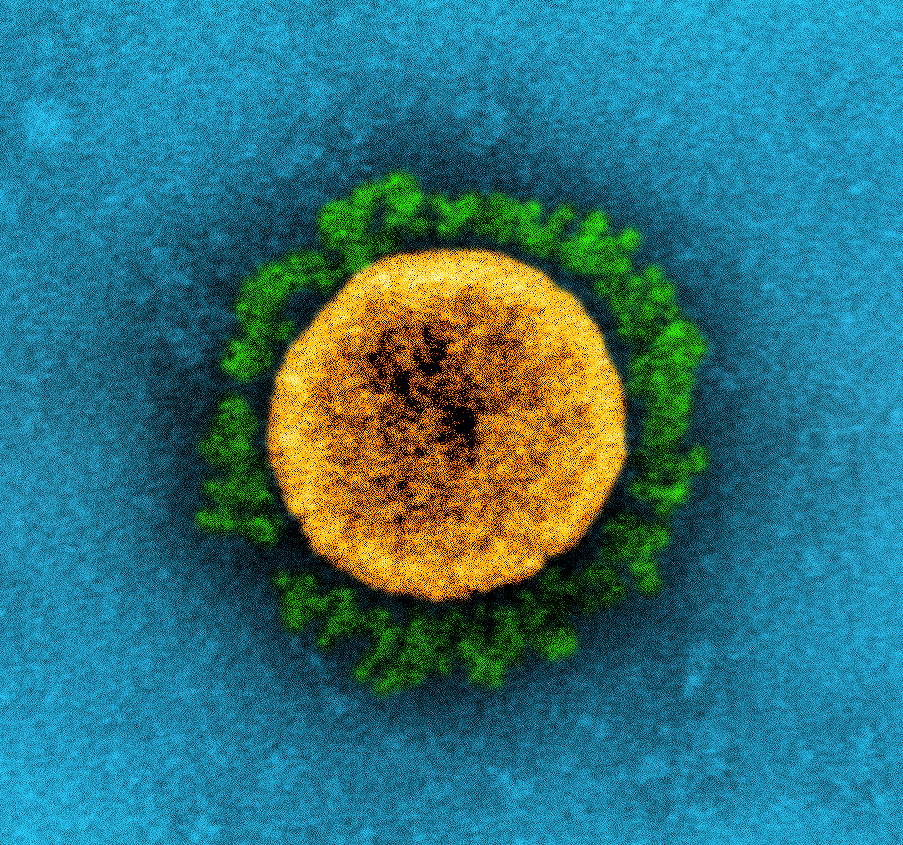
\includegraphics[width=.55\textwidth]{sarscov2micrograph}
  \caption[SARS-CoV-2 electron micrograph]{Transmission electron micrograph of a SARS-CoV-2 virus particle (UK B.1.1.7 variant), isolated from a patient sample and cultivated in cell culture. The prominent projections (green) seen on the outside of the virus particle (yellow) are spike proteins. This fringe of proteins enables the virus to attach to and infect host cells and then replicate. Image captured at the NIAID Integrated Research Facility (IRF) in Fort Detrick, Maryland.
  \textit{Figure and caption credit: NIAID}.
  }
  \label{fig:sarscov2micrograph}
\end{figure}

While the spike gene is typically considered to be under the most selective pressure, for phylogenetic analyses we will consider the entire 30kb viral genome.
\gls{sarscov2} is estimated to have a mutation rate of $1\times10^{-6}$--$2\times10^{-6}$ mutations per site per replication cycle, leading to an overall evolutionary rate of approximately $1\times10^{-3}$ substitutions per site per year, though this rate differs slightly by variant \citep{markov2023evolution}.

\subsubsection{Variants of concern}
Both the evolution and epidemiology of \gls{sarscov2} have been characterized largely by the emergence and spread of novel variants.
As the virus evolved and spread, different ``branches'' acquired mutations that resulted in variable viral fitness (Fig.~\ref{fig:sarscov2phylo}).
The most successful of these variants demonstrated enhanced transmission capabilities, immune escape properties, or both, leading to their designation by the World Health Organization as variants of concern (\gls{voc}s).
These \gls{voc}s---beginning with Alpha (first detected in the United Kingdom) in late 2020 and continuing through multiple Omicron sublineages---have repeatedly reshaped the pandemic by outcompeting their predecessors and triggering new waves of infection, even in populations who had previously achieved high levels of immunity due to infection and/or vaccination.
With very few exceptions, each novel \gls{voc} has completely outcompeted the preexisting variants, thereby driving the previous lineage to extinction (Fig.~\ref{fig:sarscov2phylo}, bottom panel).

\begin{figure}[ht]
  \centering
  \begin{subfigure}{0.9\textwidth}
    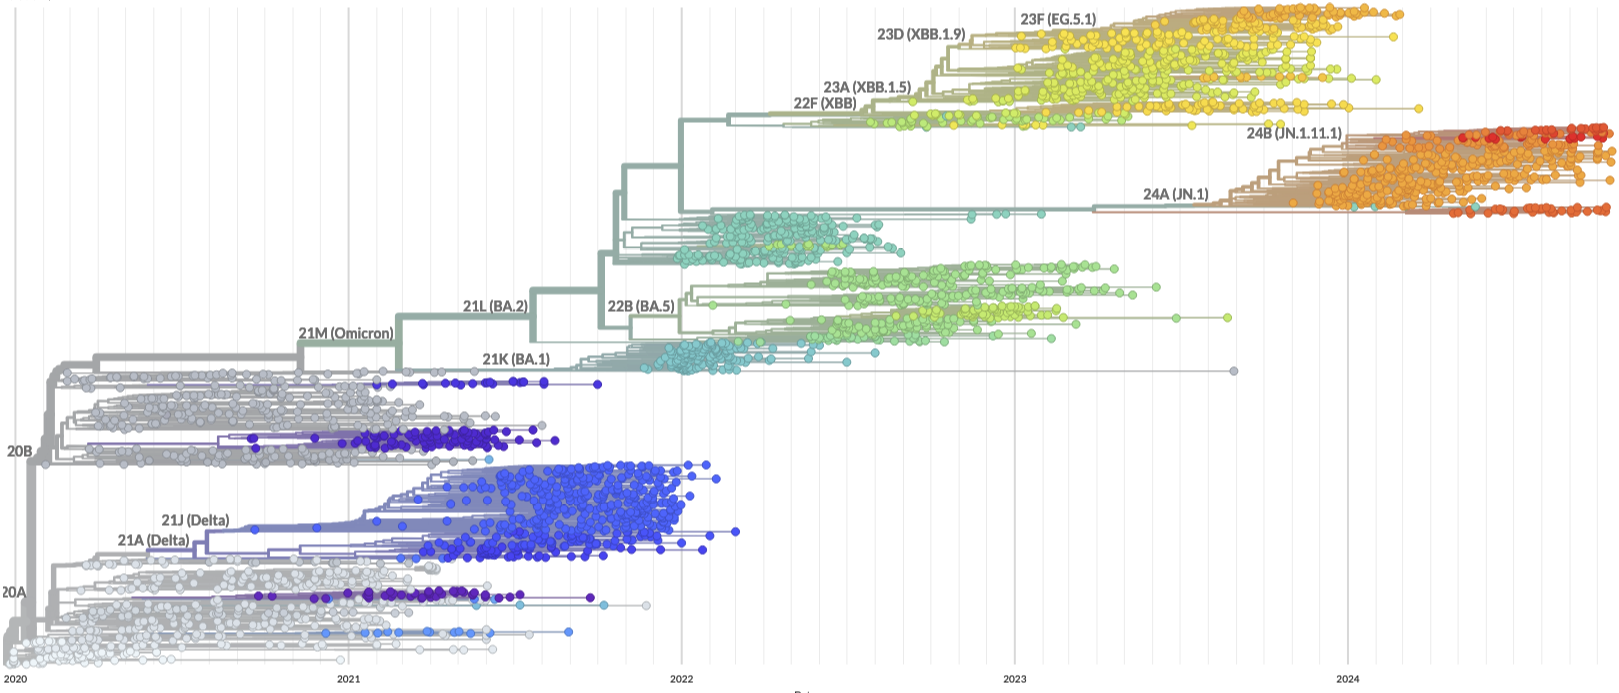
\includegraphics[width=\textwidth]{sarscov2phylogeny}
  \end{subfigure}
  \begin{subfigure}{0.9\textwidth}
    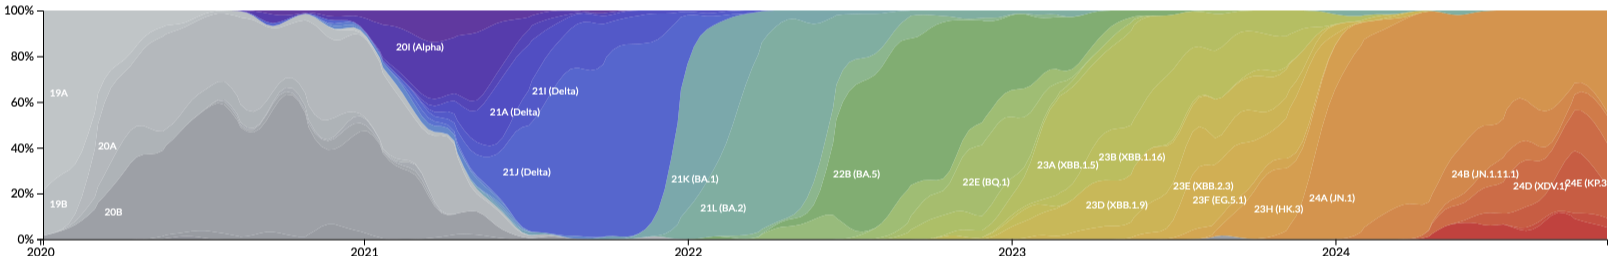
\includegraphics[width=\textwidth]{sarscov2freqs}
  \end{subfigure}
  \caption[SARS-CoV-2 phylogeny and variant frequencies]{Overview of \gls{sarscov2} variants over the course of the pandemic. \textit{(top)} Global, time-calibrated phylogenetic tree of \gls{sarscov2} sequences colored by variant spanning from the beginning of the pandemic until the present. \textit{(bottom)} estimated variant frequency plot spanning the same time period. \textit{Figure credit: nextstrain.org} \citep{hadfield2018nextstrain} (accessed 2 November 2024).}
  \label{fig:sarscov2phylo}
\end{figure}

The complexities of SARS-CoV-2 evolution demanded multiple systems for naming and tracking viral lineages.
The World Health Organization developed a simplified Greek alphabet naming system (e.g., Alpha, Delta, Omicron) for variants of concern, providing an accessible vocabulary for public health communications and media reporting.
However, more detailed classification systems were needed for scientific purposes.
The Pango nomenclature system \citep{o2021assignment,o2022pango}, which has become the \textit{de facto} standard for SARS-CoV-2 classification, uses an alphanumeric hierarchy to designate lineages (e.g., B.1.1.7, JN.1), with new levels added as the virus diversifies.
Complementing these approaches, the Nextstrain \citep{hadfield2018nextstrain,aksamentov2021nextclade} nomenclature system provides broader evolutionary context by grouping viruses into major clades (e.g., 19A, 20I) based on defining mutations.
While the WHO system names only variants with significant public health impact, these technical classification systems together provide the detailed framework necessary for tracking the full diversity of SARS-CoV-2 evolution.
A (partial) mapping between these different nomenclature systems is noted in Table~\ref{tab:variants}.
For this thesis, Pango lineages will be used primarily, however occasionally the WHO designation will also be provided.

\begin{table}[]
  \begin{tabular}{llll}
  \hline
  \textbf{WHO} & \textbf{Pango lineage} & \textbf{Nextstrain lineage} & \textbf{Time of origin} \\ \hline
  Alpha        & B.1.1.7                & 20I                         & September 2020          \\
  Beta         & B.1.351                & 20H                         & September 2020          \\
  Gamma        & P.1                    & 20J                         & September 2020          \\
  Delta        & B.1.617.2/AY           & 21A/21J                     & March 2021              \\
  Omicron      & B.1.1.529/BA/\ldots    & 21M/21F/24A/\ldots          & September 2021          \\
  \end{tabular}
  \caption{\gls{sarscov2} VOC designations, and their associated Pango and Nextstrain lineage designations. Note that there is not always an exact one-to-one correspondence as these systems use slightly different features to define distinct lineages.}
  \label{tab:variants}
\end{table}

\subsubsection{Biological and epidemiological questions}
This thesis focuses on two primary types of analysis of \gls{sarscov2}: real-time and \textit{post hoc} 

Highlight how retrospective analysis can help us understand important features of viral spread

    \subsection{Hepatitis B Virus (HBV)}
      \subsubsection{An ancient human pathogen}
      \subsubsection{HBV virology and genome}
      figure: HBV genome schematic *
      \subsubsection{Ethnospatial distribution of HBV}
      figure: HBV genotype map
      \subsubsection{Oops, no temporal signal!}
      Enter: ancient DNA
      \subsubsection{Biological and epidemiological questions}

%1.3
  \section{Phylodynamics and phylogeography}
  figure: what is a phylogeny, how to read it
  some important terms and concepts used in this thesis (just diagram out an example tree that can be used later on as well)

    \subsection{Phylogenetic inference}

      \subsubsection{Nucleotide evolution}
      models of nucleotide evolution, different substitution models
      \subsubsection{Phylogenetic likelihood}
      example: simple tree likelihood calculation on one site
      equation: tree likelihood on full multiple sites
      \subsubsection{Inferring phylogenies}
        \paragraph*{Maximum likelihood}
        \paragraph*{Bayesian inference}
        Bayes' Theorem (regular)
        Bayes' Theorem with all of the phylogenetic bits
        \paragraph*{Choosing the correct method for the questions at hand}

    \subsection{Temporal resolution and the molecular clock}
      \subsubsection{Measurably evolving populations}
      \subsubsection{Calibrating a molecular clock}
      figure: fossil calibration
      figure: prior knowledge
      figure: molecular clock inference
      \subsubsection{Temporal signal}
      figure: strong vs weak temporal signal
      \subsubsection{Clock models}
      figure: strict vs relaxed clock
      \subsubsection{Rate heterogeneity}
    \subsection{Phylodynamics and genomic epidemiology}
      \subsubsection{Population dynamics}
      \subsubsection{The coalescent}
      figure: three coalescent trees *
      comparison to case counts and calculation of $R_0$

    \subsection{Phylogeography}

      \subsubsection{Reconstructing the spatiotemporal spread of a pathogen}
      biological questions: where did it come from? where is it going? how long did it spend in a location? what are the patterns of dispersal?
      \subsubsection{Discrete trait analysis}

        \paragraph*{CTMC model of geographic dispersal in discrete space}
        figure: discrete trait phylogeography (maybe straight from Pybus \& Rambaut 2009)
        \paragraph*{Statistical power and overcoming sampling bias}
        schematic of sampling evenly through space and time and grouping samples to decrease number of locations

      \subsubsection{Other methods not used in this thesis}

        \paragraph*{Generalized linear models for discrete phylogeography}
        \paragraph*{Continuous phylogeography and spatial statistics}
        \paragraph*{Structured coalescent}

% 1.4
  \section{Phylodynamics: from theory to practice}

    \subsection{Real-time phylodynamics}
      \subsubsection{What scope of questions can we answer in real-time?}
      \subsubsection{Dataset construction: context is key}
      \subsubsection{Maximizing phylogenetic likelihood}
      \subsubsection{Public health policy relevancy and real-time communication}
      \subsubsection{The Nextstrain platform}
    \subsection{Bayesian phylodynamics}
      \subsubsection{Quantifying phylogenetic uncertainty}
      \subsubsection{Markov cahin Monte Carlo}
      figure: MCMC explanation
      \subsubsection{BEAST}
      On MCMC convergence and mixing
      \subsubsection{Prior specification}
      \subsubsection{Optimization and computational complexity}
      figure: snakemake parallelization

% Infectious diseases are now emerging or reemerging almost every year.
% This trend will continue because a number of factors, including increased global population, aging, travel, urbanization, and climate change, favor the emergence, evolution, and spread of new pathogens \citep{bloom2017emerging}.
% Many of these pathogens represent a clear and eminent threat to public health, as the ongoing corona virus disease (COVID-19) pandemic caused by severe acute respiratory syndrome corona virus 2 (SARS-CoV-2) has made brutally clear, as well as a tremendous burden on global economies.
% Other examples from the last few years include the emergence of West Nile \citep{hadfield2019twenty}, H5N1 \citep{imai2018diversity}, H1N1 \citep{bedford2015global}, Ebola \citep{dudas2017virus}, Zika \citep{fauci2016zika, faria2016zika} and Lassa \citep{kafetzopoulou2019metagenomic}.
% Demographic forces amplify the risks associated with such emerging infectious diseases (\gls{eid}).
% The global population is expected to grow to 8 billion in the near future, with nearly 60\% of the population living in relatively crowded urban areas.
% Among \gls{eid}, viral pathogens, particularly RNA viruses, stand as major concerns, owing to their high rates of nucleotide substitution and capacity to adapt to new hosts.
% Viral sequence data are invaluable for characterizing these pathogens.
% Analyzing the historical information contained in viral genomes contributes to better insight into viral emergence and early transmission dynamics, even before systematic epidemiological surveillance initiates.

% \section{Phylogenetics}

% Molecular phylogenetic inference is a particularly powerful tool available to scientists interested in inferring pathogen dynamics.
% This is a methodology by which the shared evolutionary history of a set of genomic sequences, sometimes referred to as taxa, is hypothesized based on genomic similarity.
% Phylogenetic methodologies come in many different forms, ranging from simple heuristics that approximate phylogenetic relationships based on the number of observed differences between sequences \citep{felsenstein2003inferring} to highly complex models that use demographic and geographic population structure as well as state-of-the-art models of evolution to inform phylogenetic inference \citep{dudas2018mers}.
% Additionally, phylogenetic analyses may be combined with other methodologies (e.g. methods in population genetics \citep{felsenstein2003inferring} or epidemiology \citep{black2020ten}) to provide insight into the relationship between evolutionary dynamics and other processes.
% Such processes include the dynamics of population size through time or number of migration events between geographic locations during an organism's evolutionary history.

% Phylogenetic methods can help reveal many features of a set of related taxa.
% The most frequent use of these methods is to construct a phylogenetic tree: a bifurcating (or sometimes multifurcating) representation of the inferred evolutionary history of a set of contemporary taxa---represented as tips or leaves of the tree---with inferred shared ancestors represented by internal nodes where two or more branches of the tree meet, eventually coalescing at the most recent common ancestor (\gls{mrca}) of all the taxa in a dataset.
% Such trees often use length of branches to represent genetic distance between nodes.
% A more useful representation of evolutionary history can be found by rescaling branch lengths along a tree according to a mutation rate which provides a mapping between genetic distance and time, allowing the phylogeny to be represented as a function of time.
% Phylogenetic trees can also be used to infer the shared mutation history of a set of sequences, thereby allowing the reconstruction of inferred ancestral genomes.
% Similar methods may be used to reconstruct the ancestral states of various discrete or continuous traits associated with the taxa of the tree.
% Common examples of these types of analyses include analyses of particular phenotypes of interest and phylogeographic analyses that treat sequence sampling locations as traits and aim to reconstruct the spatiotemporal spread of pathogens.
% Finally, phylogenetic methods often hypothesize a link between population dynamics and tree shape---formalized through coalescent theory \citep{Kingman1982}---whereby small populations are expected to have relatively high rates of branching (and therefore relatively short branch lengths) compared to larger populations.
% Visual examples of all of these aspects of phylodynamic analyses are illustrated in Fig.~\ref{fig:phylogeneticsOverview} \citep{pybus2009evolutionary}.



% One particularly useful application of phylogenetics is in the analysis of viral pathogen outbreaks.
% Viruses represent unique study systems for both the theoretical development of phylogenetic methodologies and the implementation of phylogenetic analyses in settings with tangible public health impact.
% In addition to their ubiquity and high profile within the human population, viruses prove highly suitable for phylogenetic inference because of their fast evolutionary rates, relatively small genomes, and frequent adherence to the assumptions of a single evolutionary history.
% Phylogenetic methods have often been used to perform \textit{post hoc} analyses of viral outbreaks, however significant work is still required before such methods can be used to inform public health responses in ``real-time'' during an ongoing epidemic.
% In this thesis, we describe phylogenetic analyses of two viral pathogens---hepatitis B virus (\gls{hbv}) and Lassa virus (\gls{lasv}).
% We use these analyses to illustrate the use of current phylogenetic and phylogeographic analysis in performing retrospective analysis, and to provide a framework for novel ``online'' phylogenetic analyses that can be performed in real-time during a viral epidemic.

% \section{Measurably evolving populations and temporal signal}

% While performing phylogenetic analyses, we are often interested in how populations evolve as a function of time, rather than as a function of genetic distance.
% To this end, we seek to correlate differences in our input data (i.e. genetic distance) with time.
% We do this by assuming that mutations accumulate along the branches of a phylogenetic tree according to some rate, which can be posited to hold a constant value across the entire phylogeny \citep{brown2011rate}, or can vary by branch according to different statistical models known as ``clock models'' \citep{drummond2006relaxed, drummond2010randomLocal}.
% We refer to this rate as an ``evolutionary rate'', generally represented in units of substitutions per site per year, which can be used to rescale the branches of a phylogeny from units of genetic distance to units of time.

% Historically, calibration of the clock models describing the evolutionary rates across branch were informed by estimates of divergence times between known lineages using fossil calibration \citep{pauling1963chemical, zuckerkandl1965molecules, near2005turtles}---a process whereby internal node times were set to an externally-supplied date of divergence.
% While this approach works well for reconstructing phylogenies for eukaryotic species whose extant genomes are more-or-less isochronous and fossil records exist to date ancient divergences, it has limited use in the inference of molecular clocks in viruses, where known divergence times may be much more limited.
% Indeed, it is frequently impossible to provide accurate prior estimates of historical divergence times, and we instead wish to infer molecular evolutionary rates directly from heterochronous (i.e. sampled a period of time) sequences.
% We call the existence of sufficient statistical power from heterochronous sequence data to determine an evolutionary rate ``temporal signal'', and we refer to a population from which we can observe a statistically significant number of mutations through time a ``measurably evolving population'' (\gls{mep}) \citep{drummond2003measurably}.
% In general, there are two sources from which we can observe \gls{mep}s: populations with available ancient genomes and rapidly evolving RNA viruses.
% Analysis of data sets that contain ancient genomes has proven to be an effective way of inferring the phylodynamics of eukaryotic populations \citep{shapiro2004bison}. %GB: if there is still room, I would be tempted to provide more information regarding this example, and perhaps the key figure from that paper
% %BP: I've not been able to think of a good way of adding this as an example without spending an inordinate amount of space. I'll add this as a backup slide in the presentation in case a question comes up.

% \section{Bayesian phylodynamic inference}

% In this thesis, I specifically aim to use Bayesian methodologies of phylogenetic inference.
% Unlike many other approaches, including fast maximum-likelihood methods, Bayesian inference does not assume that the parameters which govern statistical models take a single-point value, but rather come from a posterior probability distribution.
% Such methodologies are also informed by hypotheses of these parameter distributions provided \textit{a priori} by researchers---referred to as parameter prior distributions.
% Bayesian methodologies are particularly well suited to phylogenetic methods in several key ways.
% Firstly, they allow researchers to create estimates of evolutionary histories that account for uncertainty in the phylogenies and in other model parameters, and for which statistical support can be calculated.
% Additionally, Bayesian phylogenetic methods afford researchers the opportunity to infer many different parameters of interest (e.g. mutation rates, effective population sizes, and migration rates) jointly with the phylogeny.
% Finally, algorithms for performing Bayesian phylogenetic inference have been implemented for many different evolutionary models as a part of open-source software packages (\gls{beast}, MrBayes \citep{huelsenbeck2001mrbayes}) allowing tractable computation of complex datasets. %BP: updated to address poorly worded previous version.

% To perform Bayesian (phylodynamic) inference it's frequently necessary to compute high-dimensional integrals to produce exact posterior distributions, a task that's unfortunately analytically intractable in nearly all but the simplest of situations.
% However, this hurdle can be overcome by simulating a Markov chain whose stationary distribution is the desired posterior distribution.
% This approach is known as Markov chain Monte Carlo (\gls{mcmc}) and can be exploited to numerically approximate posterior distributions of phylogenetic models.

% The implementation of such methods typically works according to the Metropolis-Hastings algorithm \citep{metropolis1953equation, hastings1970monte}.
% First, a starting value for each parameter of interest---including the initial tree topology---is randomly drawn from its prior distribution or set to pre-specified values
% We call this parameter set $\mathbf{\theta}$.
% A new ``proposal'' set, $\mathbf{\theta^\prime}$, is then generated by stochastically perturbing the original parameter set according to various parameter-specific transition kernels with probability $g(\mathbf{\theta^\prime}\vert\mathbf{\theta})$.
% A likelihood for the model can then be calculated for both the initial parameter set, $L(\mathbf{\theta})$, and the proposal set, $L(\mathbf{\theta^{\prime}})$.
% The ratio of each likelihood to its associated parameter probabilities is used to define an acceptance probability, $A$, for that parameter set such that the acceptance ratio of the initial set is $A(\mathbf{\theta}, \mathbf{\theta^{\prime}})=\frac{L(\mathbf{\theta})}{g(\mathbf{\theta}\vert\mathbf{\theta^\prime})}$ and the acceptance ratio for the proposal set is $A(\mathbf{\theta^\prime}, \mathbf{\theta})=\frac{L(\mathbf{\theta^\prime})}{g(\mathbf{\theta^\prime}\vert\mathbf{\theta})}$.
% The new proposal set is accepted with probability proportional to the ratio of these acceptance probabilities:
% $$
% \frac{A(\mathbf{\theta}, \mathbf{\theta^{\prime}})}{A(\mathbf{\theta^\prime}, \mathbf{\theta})} = min(1,\frac{L(\mathbf{\theta^\prime})}{L(\mathbf{\theta})}\frac{g(\mathbf{\theta}\vert\mathbf{\theta^\prime})}{g(\mathbf{\theta^\prime}\vert\mathbf{\theta})}).
% $$
% That is, if the proposal set yields a higher acceptance probability than the initial set, it is accepted as the new parameter set, and if it has an acceptance probability lower than the initial candidate set, it will be accepted with probability proportional to the ratio of the two acceptance probabilities.
% This process is then repeated until a stable parameter set is reached.
% This stable set is considered to be the posterior distribution from which we would like to sample.
% Once this stable set is found, the same process is continued, with the state of the chain recorded at regular intervals, until the posterior has been sufficiently explored.
% At that stage, which can take days or even weeks to reach (but see section~\ref{sec:ess}), we can stop our Bayesian analysis and construct summaries of all parameters of interest.

% \subsection{Statistical and computational challenges}

% One of the major challenges of phylogenetic inference that can lead to very time-consuming analyses is the vast size of the state space of potentially inferred variables.
% The size of ``tree space''---the set of all possible phylogenetic trees for a given dataset---scales at the rate $\frac{(2n-3)!}{2^{n-1}(n-1)!}$.
% This is far too large to exhaustively explore for the datasets that researchers are typically interested in; for a dataset consisting of only thirty taxa, the number of possible rooted, labeled phylogenies totals over $10^{38}$ \citep{felsenstein2003inferring}.
% For the datasets that we explore in this thesis---ranging in size to 769 taxa---this number grows to vastly overshadow the number of atoms in the observable universe.
% As such, exhaustively exploring this space is impossible, and traversing this space algorithmically can still take considerable time.

% \subsection{Effective sample size and burn-in}
% \label{sec:ess}

% Bayesian phylogenetic inference of large, complex datasets can hence take upwards of a month of constant computational time before a chain achieves convergence and has adequately explored the full posterior distribution.
% During this time, the constructed Markov chain is sampled at fixed intervals by recording the state of all parameters of the chain.
% How thoroughly the posterior has been sampled can be quantified using a metric known as the effective sample size (\gls{ess})---a measure of the number of effectively independent draws from the posterior distribution that the Markov chain sample is equivalent to.
% Because sequential samples of the chain's state are frequently highly correlated, the \gls{ess} is an appropriate metric for how fully the \gls{mcmc} has explored the posterior distribution of interest.
% While there is no theoretical foundation for using a specific cut-off value when computing the \gls{ess}, a commonly applied consensus is to accumulate \gls{ess} values over 200 for each parameter of interest as a decent trade-off between length of computation and the number of independent samples collected for a specific parameter.

% A significant amount of computation time is consumed by the chain moving from its starting point in state space toward the posterior distribution---a period referred to as the ``burn-in''.
% Because the chain aims to rapidly traverse parameter space towards the posterior, this initial burn-in phase does not help to accumulate independent samples from said posterior and hence the entire burn-in period is discarded prior to summarizing the results from the analysis.
% A major computational issue stemming from the burn-in period is that the time spent in burn-in can only be mitigated by either specifying prior distributions that are strongly informative of the posterior distribution, or by designing novel transition kernels to move towards the posterior in a more efficient manner.
% This means that even if identically parameterized chains are run in parallel the burn-in period must take place for each independent run, significantly lowering the utility of chain-level parallelization.

% \subsection{BEAST}

% For the analyses described in this thesis, I make use of the software package Bayesian Evolutionary Analysis Sampling Trees (\gls{beast}) 1.10 \citep{suchard2018bayesian}.
% \gls{beast} is an easy-to-use software package in which many Bayesian phylogenetic models---and their associated priors and transition kernels---have been implemented and optimized such that analyses on large datasets may be easily specified and run efficiently on a wide variety of computing resources.
% This tool mostly implements Bayesian phylogenetic inference via \gls{mcmc}.
% Recent developments have started exploring the use of Hamiltonian Monte Carlo approaches to speed computation times and ensure more thorough exploration of state space.
% Analyses in \gls{beast} are facilitated by hardware optimization libraries such as BEAGLE \citep{ayres2019beagle}, as well as a large suite of utility programs that make running analyses in parallel and quickly interpreting results feasible.

% \section{Viral pathogens}
% Viral pathogen outbreaks are a particularly useful study system for Bayesian phylogeneticists because their relatively small genomes typically allow for tractable computation.
% The rapidity with which viruses move though populations and their fast evolutionary rates give many viral pathogens rather strong temporal signal, and therefore make them good candidates for Bayesian phylogenetic inference.
% Viral pathogens make interesting study systems because of the large influence that they exert on human quality of life.
% Viruses frequently cause human suffering and death, both as endemic diseases (seasonal influenza, hepatitis, etc.) and the agents behind sudden disease epidemics (Zika, Ebola, Lassa).
% Indeed, viruses have been responsible for the majority of the most deadly pandemics of the last century (1918 Spanish influenza, 2009 Swine flu, COVID-19).
% Even when they do not cause large-scale epidemics or global pandemics, or when they do not cause death, viruses can still cause vast amounts of human suffering though localized, small-scale outbreaks that cause severe health problems for those that they infect.
% In this thesis, we present the results of Bayesian phylogenetic analyses of two separate viral pathogens: hepatitis B virus (\gls{hbv}) and Lassa virus (\gls{lasv}).
% Here, we provide some information regarding the genome structure of these two pathogens, which will aid in justifying modeling assumptions in subsequent chapters.


% \subsection{Hepatitis B virus (HBV)}

% \gls{hbv} has infected over two billion people worldwide and puts over 350 million people at risk of cirrhosis and liver cancer \citep{kane1995global}.
% The virus is classified into eight different genotypes based on genomic sequence divergence.
% These genotypes show strong ethnospatial patterns and are often correlated directly to the region of the world where they are most prominent \citep{schaefer2007hepatitis}.
% \gls{hbv} consists of two partially overlapping strands of DNA (Fig.~\ref{fig:hbvGenome}).
% The long strand ranges from 3,020--3,320 bases in length, while the short strand ranges from 1,700--2,800 nucleotides long, depending on genotype \citep{kay2007hepatitis}.



%%%%%%%%%%%%%%%%%%%%%%%%%%%%%%%%%%%%%%%%%%%%%%%%%%
% Keep the following \cleardoublepage at the end of this file,
% otherwise \includeonly includes empty pages.
\cleardoublepage

% vim: tw=70 nocindent expandtab foldmethod=marker foldmarker={{{}{,}{}}}
